% pdflatex 0_lustrik_doktorat; bibtex 0_lustrik_doktorat; pdflatex 0_lustrik_doktorat; pdflatex 0_lustrik_doktorat
% or run: runlatex.bat

\documentclass[a4paper, 12pt, oneside]{article}
% \setlength{\parskip}{1 cm} %space between paragraphs

\usepackage{graphicx}
\usepackage[utf8]{inputenc}
\usepackage[slovene]{babel} %adds slovene chars
\usepackage{booktabs} %advanced tables
\usepackage{array}
\usepackage{fancyhdr}
\usepackage{Sweave}
\usepackage[tmargin=35mm, bmargin=30mm, lmargin=30mm, rmargin=25mm]{geometry} %custom margins
\usepackage[font=footnotesize, justification=raggedright,tablename=Preglednica]{caption}
\usepackage{subcaption}
\usepackage[Q=yes, url=yes]{examplep} %this is for verbatim inline text, you can insert
\usepackage{longtable}
\usepackage{natbib}  % some extra cookies for bibtex
\usepackage[table]{xcolor}
\usepackage{float}
\usepackage{appendix}
\usepackage{setspace}
\usepackage[T1]{fontenc} %tole rabiš, da lahko nardiš CAPS in BOLD hkrati - ma ne dela, mona
\usepackage[hidelinks]{hyperref}
\usepackage[justification=justified]{caption}
\usepackage{amsmath} % matrices?
\usepackage[tiny, md]{titlesec} % change sectioning
\usepackage[titles]{tocloft} % add Figure/Table to list of figures/tables
\usepackage{titletoc}
\usepackage{epigraph}

% This chunk controls  space between sections, subsections..., and figures in TOC.
\renewcommand{\cftsecafterpnum}{\vspace{-10pt}} % reduces space between paragraphs in toc
\renewcommand{\cftsubsecafterpnum}{\vspace{-8pt}}
\renewcommand{\cftsubsubsecafterpnum}{\vspace{-8pt}}
\renewcommand{\cftparaafterpnum}{\vspace{-8pt}}

\setlength{\epigraphwidth}{0.5\textwidth}
\setlength{\epigraphrule}{0pt}
\setlength{\beforeepigraphskip}{4cm}

% help pictures that they're not alone on a page
\renewcommand{\topfraction}{0.85}
\renewcommand{\textfraction}{0.1}

% add Figure/Table: x to LOF, TOF (titletoc)
%figure
\contentsmargin{0.5cm}
\titlecontents{figure}
  [1.7cm]
  {}
  {\makebox[0pt][r]{%
      \makebox[1.7cm][l]{Slika~\thecontentslabel:}%
    }%
  }
  {\hspace{-1.7cm}}
  {\titlerule*[6pt]{.}\contentspage}

% table
\contentsmargin{0.5cm}
\titlecontents{table}
  [2.75cm]
  {}
  {\makebox[0pt][r]{%
      \makebox[2.75cm][l]{Preglednica~\thecontentslabel:}%
    }%
  }
  {\hspace{-2cm}}
  {\titlerule*[6pt]{.}\contentspage}

% redefine section, subsection, subsubsection and subsubsubsection
\titleformat{\section}{\normalfont\fontfamily{cmr}\fontsize{12}{1.2em}\bfseries}{\thesection}{1ex}{}
\titleformat{\subsection}{\normalfont\fontfamily{cmr}\fontsize{12}{1.2em}}{\thesubsection}{1ex}{}
\titleformat{\subsubsection}{\normalfont\fontfamily{cmr}\fontsize{12}{1.2em}\bfseries}{\thesubsubsection}{1ex}{}
\titleformat{\subsubsubsection}{\normalfont\fontfamily{cmr}\fontsize{12}{1.2em}}{\thesubsubsubsection}{1ex}{}

%header defs
\pagestyle{fancy}
\addtolength{\headheight}{\baselineskip}
\lhead{\footnotesize\textup{Luštrik R. \naslov .} \\
   \hspace{1cm} Dokt. disertacija, Ljubljana, Univ. v Ljubljani, Biotehniška fakulteta, 2019}
\rhead{\thepage}
\fancyfoot{} %clear footers

%misc settings
\setlength{\parindent}{0in} %no indentation throughout the document

\newcommand{\avtor}{Roman \textsc{Luštrik}} %vstavi ime diplomanta (that's you)
\newcommand{\naslov}{Modeli s prostorsko omejitvijo za ocenjevanje gostote superpopulacije} %vstavi naslov diplomskega dela
\newcommand{\naslovEN}{Spatially explicit modeling of superpopulation density} %vstavi angleški naslov diplomskega dela

\newcommand{\platnica}{\textsc{\MakeUppercase{\textbf{\naslov}}}}
\newcommand{\platnicaEN}{\MakeUppercase{\textbf{\naslovEN}}}

%custom hyphenation
\hyphenation{la-bo-ra-to-rij-sko po-i-men-o-van-je} %separate words with space

%little something for natbib
\citestyle{egu}
\setlength{\bibhang}{1cm}
\addto{\captionsslovene}{
  \renewcommand*{\refname}{}
}

% add extra sub section
% \newcommand{\subsubsubsection}[1]{\paragraph{#1}\mbox{}\\}
\newcommand{\subsubsubsection}[1]{\paragraph{#1} ~\\[1.2em]}
\setcounter{secnumdepth}{4}
\setcounter{tocdepth}{4}

\setlength{\LTcapwidth}{23cm} %podaljšanje caption-a

\author{Roman Luštrik}

% reduce spacing between sections
\titlespacing{\section}{0pt}{\parskip}{\parskip}
\titlespacing{\subsection}{0pt}{\parskip}{\parskip}
\titlespacing{\subsubsection}{0pt}{\parskip}{\parskip}
\titlespacing{\subsubsubsection}{0pt}{\parskip}{\parskip}
\setlength{\parskip}{1em} % reduce spacing between paragraphs

% rename table caption name
% \renewcommand{\tablename}{Preglednica}

\begin{document}

% platnica
\begin{titlepage}
\voffset -2cm
\enlargethispage{2cm}
\begin{center}
\Large\textsc{Univerza v ljubljani} \\
\Large\textsc{Biotehniška fakulteta} \\
%\Large \textsc{Oddelek za biologijo} \\
\vspace{7cm}
\Large\avtor \\
\vspace{2cm}
\LARGE\platnica \\
\vspace{2cm}
\Large \textsc{Doktorska disertacija}\\
\vspace{8cm} %this may need adjusting due to title length
\Large Ljubljana, 2019 \\
\end{center}
\end{titlepage}

% naslovna stran
\begin{titlepage}
\voffset -2cm
\enlargethispage{2cm}
\begin{center}
\Large\textsc{Univerza v ljubljani}\\
\Large\textsc{Biotehniška fakulteta}\\
\vspace{6cm}
\avtor \\
\vspace{1cm}
\large \platnica\\
\vspace{0.8cm}
\textsc{Doktorska disertacija}\\
\vspace{2cm}
\large\platnicaEN\\
\vspace{0.8cm}
\textsc{Doctoral dissertation}\\
\vspace{8cm} %this may need adjusting due to title length
\Large Ljubljana, 2019 \\
\end{center}
\end{titlepage}

\begin{titlepage}
\epigraph{In god we trust, all others bring data.}{-- W. Edward Deming}
\epigraph{If we have data, let’s look at data. If all we have are opinions, let’s go with mine.}{-- Jim Barksdale}
\end{titlepage}

%page number 2 - the presiding commission
\newpage
\pagenumbering{Roman}
\setcounter{page}{2}

Na podlagi Statuta Univerze v Ljubljani ter po sklepu Senata Biotehniške fakultete in sklepa 44. seje Komisije za doktorski študij Univerze v Ljubljani z dne 13. 11. 2013 (po pooblastilu Senata Univerze z dne 20. 1. 2009) je bilo potrjeno, da kandidat izpolnjuje pogoje za opravljanje doktorata znanosti na Interdisciplinarnem doktorskem študijskem programu Statistika. Za mentorja je bil imenovan prof. dr. Andrej Blejec. S sklepom Senata UL z dne 13. 1. 2018 je bil za novega mentorja imenovan doc. dr. Tomaž Skrbinšek.

\vspace{4cm}

Komisija za oceno in zagovor:\\

\begin{table}[!ht] %[ht] means ``position this float HERE at the TOP''
 \begin{tabular}{>{\raggedright} m{4cm} m{10cm}}
   Predsednik: & prof. dr. Andrej \textsc{Blejec} \par Univerza v Ljubljani, Biotehniška fakulteta, Oddelek za biologijo \\ [10pt]
   Član: & prof. dr. Janez \textsc{Stare} \par Univerza v Ljubljani, Medicinska fakulteta, Inštitut za biostatistiko in medicinsko informatiko \\ [10pt]
   Članica: & doc. dr. Martina \textsc{Lužnik} \par Univerza na Primorskem, Fakulteta za matematiko, naravoslovje in informacijske tehnologije, Oddelek za biodiverziteto \\ [10pt]
 \end{tabular}
\end{table}

\vspace{3cm}

Datum zagovora:

\begin{flushright}
\avtor
\end{flushright}

\newpage
%ključna dokumentacijska informacija, vsebina strani naj ne presega ene strani
\section*{KLJUČNA DOKUMENTACIJSKA INFORMACIJA (KDI)}
\addcontentsline{toc}{section}{KLJUČNA DOKUMENTACIJSKA INFORMACIJA (KDI)}

% KDI variables
\newcommand{\numroman}{X}
\newcommand{\numpages}{55}
\newcommand{\numtables}{1}
\newcommand{\numfigs}{11}
% \newcommand{\numsup}{0}
\newcommand{\numsources}{67}

% navodila za oblikovanje: http://www.bf.uni-lj.si/fileadmin/users/1/knjiznice/Navodila_za_pripravo_zakljucnih_pisnih_izdelkov_na_BF.pdf
\begin{table}[H]
 \begin{tabular}{>{\raggedright} p{2cm} m{12.5cm}}
  ŠD & Dd \\
  DK & UDK 519.22:57(043.3) \\
  KG & populacije, gostota, ocena velikosti populacije, učinek roba, metoda lova-ponovnega ulova, program MARK, program R \\
  AV & \textsc{Luštrik}, Roman, univ. dipl. biol. \\
  SA & \textsc{Skrbinšek}, Tomaž (mentor) \\
  KZ & SI-1000 Ljubljana, Jamnikarjeva 101 \\
  ZA & Univerza v Ljubljani, Biotehniška fakulteta, Interdisciplinarni doktorski študijski program Statistika \\
  LI & 2019 \\
  IN & \textsc{\naslov} \\
  TD & Doktorska disertacija \\
  OP & \numroman, \numpages~str., \numtables~pregl., \numfigs~sl., \numsources~vir. \\ %št. rimskih strani, št. navadnih strani, št. preglednic, kart, prilog in virov
  IJ & sl \\
  JI & sl/en \\
  AI & Eden od načinov ocenjevanja velikosti populacij je z uporabo metod lova-ponovnega ulova. Metoda predpostavlja, da je populacija zaprta (ni rojstev, smrti, priseljevanja in odseljevanja) in da imajo vsi osebki enako verjetnost ulovljivosti. Ker populacij pogosto ne moremo vzorčiti v celoti, zaradi prehoda roba območja vzorčenja prihaja do kršenja teh dveh predpostavk, kar imenujemo učinek roba. Klasični Hugginsov model za zaprte populacije za oceno parametrov sam po sebi ne omogoča uporabe prostorskih statistik, omogoča pa vključevanje individualne spremenljivke. V tem delu s pomočjo simulacij testiramo učinkovitost vključevanja individualne spremenljivke v model z namenom odpravljanja posledic učinka roba. Ugotovili smo, da je model, ki vključuje prostorsko informacijo, boljši od modela, ki te informacije ne nosi. Razlika v ocenjenem parametru verjetnosti ulovljivosti ($\hat{p}$) je s praktičnega vidika zelo majhna. Pristranskost ocene parametra $\hat{p}$ je najmanjša za tiste simulacije, kjer je velikost domačega okoliša znatno manjša od velikosti območja vzorčenja, za ostale pa je močno pristranska. Pristranskost ocene parametra $\hat{p}$ se pozna tudi pri oceni gostote, ki je zelo pristranska za primere, kjer je domač okoliš velik v primerjavi z velikostjo območja vzorčenja. Na podlagi porazdelitve za izračun individualne spremenljivke smo povečali območje vzorčenja in uspeli do neke mere popraviti gostoto, a le ob predpostavki, da imamo na voljo reprezentativno obliko in velikost domačega okoliša.\\ %  ~200 besed
 \end{tabular}
\end{table}

\newpage
%keywords documentation
\section*{KEY WORDS DOCUMENTATION (KWD)}
\addcontentsline{toc}{section}{KEY WORDS DOCUMENTATION (KWD)}

\begin{table}[H]
  \begin{tabular}{>{\raggedright} p{2cm} m{12.5cm}}
  DN & Dd \\
  DC & UDC 519.22:57(043.3) \\ %decimalna klasifikacija (UDK ali GDK)
  CX & populations, density, population size estimate, edge effect, mark-recapture, program MARK, program R \\
  AU & \textsc{Luštrik}, Roman \\
  AA & \textsc{Skrbinšek}, Tomaž (mentor) \\
  PP & SI-1000 Ljubljana, Jamnikarjeva 101 \\
  PB & University of Ljubljana, Biotechnical Faculty, Interdisciplinary Doctoral Programme in Statistics \\
  PY & 2019 \\
  TI & \textsc{\naslovEN} \\
  DT & Doctoral dissertation \\
  NO & \numroman, \numpages~p., \numtables~tab., \numfigs~fig., \numsources~ref.\\ %št. rimskih strani, št. navadnih strani, št. preglednic, kart, prilog in virov
  LA & sl \\
  AL & sl/en \\
  AB & Among methods for estimating population sizes, mark-recapture is a popular choice. It assumes population closure (void of deaths, births, immigration and emigration) and equal probability of capture. Since populations often cannot be encompassed entirely, some individuals cross in and out of the sampling area in violation of aforementioned assumptions, which is termed edge effect. The time-tested Huggins model does not in itself use spatial information to estimate parameters; however, it does enable use of an individual covariate. In this thesis, we use simulations to test whether including spatial information through an individual covariate helps alleviate edge effect. Our findings suggest that including spatial information does improve the model. For practical purposes, the difference in estimates of probability of capture ($\hat{p}$) between models is negligible. Bias of $\hat{p}$ is smallest in cases where home range size is small relative to sampling area size and large for cases where home range is comparatively large. This is also evident in density estimates, which are highly biased in cases where home range is relatively large compared to sampling area. We increased the sampling area radius based on distributions used to calculate the individual covariate and managed to somewhat alleviate the bias, provided that the calculated home range shape and size are representative.\\
  \end{tabular}
\end{table}

\newpage

% Table of contents
\renewcommand*{\contentsname}{}
\section*{\textbf{\large KAZALO VSEBINE}}
\vspace{-1.8cm}
\addcontentsline{toc}{section}{\textbf{KAZALO VSEBINE}}
\renewcommand{\baselinestretch}{0.8}\normalsize
\tableofcontents
\renewcommand{\baselinestretch}{1.0}\normalsize

% List of tables
\newpage
\normalsize
\renewcommand*\listtablename{}
\section*{\textbf{KAZALO PREGLEDNIC}}
\vspace{-1.5cm}
\addcontentsline{toc}{section}{\textbf{KAZALO PREGLEDNIC}}
\listoftables

% List of images
\newpage
\normalsize
\renewcommand*\listfigurename{} % remove list of figures title
\section*{\textbf{KAZALO SLIK}} % add title manually
\vspace{-1cm}
\addcontentsline{toc}{section}{\textbf{KAZALO SLIK}} % manually add it to LOC
% \renewcommand{\baselinestretch}{0.4}\normalsize
\listoffigures
% \renewcommand{\baselinestretch}{1.0}\normalsize

\newpage
\section*{OKRAJŠAVE IN SIMBOLI}
\addcontentsline{toc}{section}{\textbf{OKRAJŠAVE IN SIMBOLI}}

\begin{table}[H]
 \begin{tabular}{>{\raggedright} p{2cm} m{12cm}}
   $p$ ($\hat{p}$), $c$ & Verjetnost ulovljivosti (in njena cenilka) v kontekstu Hugginsovega modela za zaprte populacije \\
   $M_0$ & Model, kjer smo predpostavili, da je ulovljivost enaka za prvo in vse nadaljnje ulove \\
   $M_{sp}$ & Model, kjer smo predpostavili heterogenost ulovljivosti. To heterogenost opišemo s pomočjo individualne spremenljivke \\
   CAPWIRE & Model za ocenjevanje velikost populacije, ki predpostavlja različno število skupin osebkov z enakim $p$ \\
   TIRM & Ena oblika modela CAPWIRE \\
   $D$ ($\hat{D}$) & Ocenjena gostota populacije in njena cenilka \\
   AICc & Akaikov informacijski kriterij s popravkom za male vzorce \\
 \end{tabular}
\end{table}
\normalsize

\pagenumbering{arabic}
\section{Uvod}
Velikosti populacije je v ekologiji pomemben parameter, ki ga lahko preučujemo. Služi v pomoč pri raziskovanju drugih značilnosti populacije. Z nekaterimi populacijami živali aktivno upravljamo in ocena številčnosti je lahko izhodiščni parameter za kvaliteten trajnostni odvzem osebkov iz populacije.

\subsection{Pomen ocene velikosti populacije kot biološki parameter}
Populacijo lahko opredelimo kot skupino osebkov iste vrst, ki naseljujejo skupni prostor v danem času \citep{krebs_ecology:_2001}. Kot taka je na voljo za proučevanje in upravljanje.

Proučevanje katero koli populacije se začne s poznavanjem njene biologije in ekologije. Posamično ali v skupinah proučujemo demografske parametre, ki dajo vpogled v populacijo in vrsto. Taki parametri so denimo življenjska doba, število potomcev, stopnja preživetja različnih starostnih skupin ipd. Poleg teh pa je pomembna tudi velikosti populacije, ki jo lahko imenujemo tudi številčnost oz. jo gledamo na znano velikem prostoru kot gostoto. Številčnost je eden najbolj intuitivnih parametrov, ki jih lahko pripišemo populaciji, saj predstavlja izhodišče za upravljanje. Poleg številčnosti so lahko drugi omejujoči dejavniki, denimo genetska slika. Primera takih dveh (sub) populacij lahko spremljamo na primerih floridskega panterja \citep{pimm_genetic_2006} ali nenazadnje slovenskega risa.

\subsection{Načini ocenjevanja številčnosti}
Velikost populacije lahko ocenjujemo na dva načina. Kot število osebkov na območju vzorčenja ali neposredno kot gostoto (število osebkov na prostorsko enoto). V obeh primerih pa ostaja problem zaznavnosti posameznega osebka. Zaradi načina življenja ali pa velikega območja na katerem se populacija razteza, vseh živali fizično ni mogoče zaznati v izvedljivih časovnih, finančnih in drugih okvirih. Zato moramo poseči po pristopih, ki omogočajo, da zaznanim osebkom "prištejemo" tiste, ki smo jih spregledali. Na ta način lahko ocenimo vsoto zaznanega in pričakovanega dela populacije. S pomočjo znanstveno preverljivih metod lahko oceni podamo tudi interval zaupanja, s katerim lahko sporočimo tudi kako natančna je naša ocena.

Ko na določenem območju z gotovostjo zaznamo vse osebke, jih preprosto preštejemo. To imenujemo cenzus, kjer predpostavimo, da vse osebke zagotovo zaznamo ($p=1$). Cenzusi v ekologiji niso pogosti, ker določen delež osebkov navadni ni mogoče zaznati. Metode, ki upoštevajo dejstvo, da vsi osebki med vzorčenjem niso zaznani s popolno gotovostjo ($p < 1$), so osnovane na podlagi štetja na ploskvah, oddaljenosti od opazovalca in lova in ponovnega ulova \citep{williams_analysis_2002}.

Metoda štetja na ploskvah deluje na način, da območje, kjer želimo oceniti številčnost neke populacije, razdelimo na prostorske podenote. Na vzorcu podenot izvedemo vzorčenje in iz ocen številčnosti v podenotah lahko sklepamo o številčnosti na večjem območju. Pri tem moramo upoštevati več predpostavk, saj ima sklepanje iz vzorca na večje območje več pasti.

Metode, kjer se beleži oddaljenost osebka od točke opazovanja, v prvi vrsti podajo oceno gostote. Opazovanje lahko poteka na naključno izbranih točkah ali transektih, vhodni podatki za računanje pa je razdalja osebka do transekta. Predpostavlja se, da je na transektih, ki jih popisovalec pregleduje, zaznavnost 1, z oddaljenosti od transekta pa zaznavnost pada po krivulji. Tip krivulje lahko izberemo na podlagi teorije ali prakse.

Do sedaj opisani načini za oceno številčnosti niso upoštevali identitete zaznanega osebka, kar pa je domena metod ulova in ponovnega ulova.

\subsection{Metoda lova in ponovnega ulova}
\subsubsection{Osnovne značilnosti metode lova in ponovnega ulova}

Metode ulova in ponovnega ulova se od zgoraj naštetih metod razlikujejo po tem, da za informacijo uporabljajo identiteto osebka. Zanesljiva določitev identitete osebka je najvišja kvaliteta podatka, ki ga lahko pridobimo za oceno številčnosti populacije. Kljub temu, da so bile nekatere matematične osnove metode lova in ponovnega ulova razvite že pred več stoletji, se je paleta modelov razširila in prešla v splošno uporabo v začetku dvajsetega stoletja \citep{pollock_capture-recapture_2000}.

Poznamo več matematičnih modelov in vsak ima svoje značilnosti. V eni od delitev lahko modele razvrstimo na dve večji skupini, ki se razlikujeta po tem, da so primerne za odprte oz. zaprte populacije. O odprtih populacijah govorimo takrat, ko osebki med vzorčenjem prihajajo in odhajajo iz populacije. Zaprte populacije tega prehoda ne predpostavljajo in je zato že v osnovi pojem "velikost populacije" lažje opredeliti. Pregled metod za zaprte populacije v svojem klasičnem delu opišejo \citet{otis_statistical_1978}, kasneje pa še drugi (tudi za odprte), kot so \citet{white_capture-recapture_1982}, \citet{seber_review_1986} in \citet{white_program_1999}.

\subsubsection{Prepoznavanje osebkov}
Da lahko osebek prepoznamo kot edinstvenega, ga moramo na nekakšen način ujeti oz. zaznati. V preteklosti je to predstavljalo fizičen ulov, nakar so žival nedvoumno označili. Osebke se označuje na načine, da je oznaka trajna ali začasna (npr. označevanja robnih lusk ščita pri želvah \citep{pike2005}, ščipanje ušes ali nohtov pri manjših sesalcih \citep{wiewel_assessing_2007}, pisanje številk na krila metuljev \citep{jugovic_movement_2017}, ščipanje prstov pri dvoživkah \citep{campbell_evaluation_2009}, opremljanje z ušesnimi značkami, barvanje kožuha, tetoviranje idr.).

Z napredovanjem molekularnih tehnik in večanjem računalniške moči, je danes možen ulov brez fizičnega stika z osebki. Tako je manj verjetno verjetno, da bo spremenila vedenje in posledično spremenila njeno ulovljivost.
Iz neinvazivno nabranih vzorcev (npr. sluzi, sline, dlake, iztrebka, perja) preko DNK z relativno visoko zanesljivostjo določimo identiteto osebka. Pri živalih, ki imajo značilno obarvano kožo ali dlako (npr. trebuh nekaterih dvoživk, obarvanost kožuha pri risu), lahko s pomočjo fotografij in računalniških programov ločimo med različnimi osebki.

\subsubsection{Območje vzorčenja}
Ulov in označevanje osebkov poteka na geografsko določenem območju, ki za živali z velikim območjem gibanja le deloma zaobjame proučevano populacijo. Velikost območja vzorčenja je navadno omejeno zaradi velikih razdalj potovanj, fizičnimi mejami (otoki) ali pa s političnimi mejami (parkov, držav ali drugih enot). Iz tega sledi, da osebke zaznavamo (lovimo), njihovo gibanje ni nujno omejeno na naše arbitrarno določeno območje vzorčenja.

\subsubsubsection{Domač okoliš}
Območje domačega okoliša osebka predstavlja prostor, kjer se zadržuje osebek med dnevnimi aktivnostmi. Raba prostora navadno sovpada s trenutnimi potrebami osebkov (iskanje hrane, partnerjev) in se v času lahko spreminja. Velikost območja je odvisna od velikosti organizma ter razpoložljivosti hrane in drugih virov potrebnih za življenje.

\subsubsubsection{Superpopulacija}
Populacija je skupina osebkov, ki se nahajajo znotraj območja vzorčenja. Poleg osebkov, ki se neprestano zadržujejo znotraj območja vzorčenja, lahko zaznamo tudi osebke, ki prehajajo njegove meje, ker se njihov domač okoliš le deloma prekriva z našim arbitrarnim območjem vzorčenja. Njihova zaznavnost je v povprečju nižja od osebkov, ki se v prostoru in času stalno nahajajo v območju vzorčenja. Skupaj z ostalimi osebki tvorijo t.i. superpopulacijo, za katero pa ne vemo natančno kako je prostorsko omejena.


\subsubsection{Predpostavke metod ulova in ponovnega ulova}
Kot velja za vse modele, tudi pri modelih ulova in ponovnega ulova veljajo predpostavke. Kršitev le-teh ima lahko za posledico blage ali hude posledice. V splošnem se trudimo, da predpostavkam zadostimo. V primerih simuliranih vrednosti lahko nekatere predpostavke zanemarimo ali pa jih celo nadzorujemo, kar nam pomaga proučevati kaj se dogaja pri kršenju le-teh.

\subsubsection{Zanesljivost označevanja}
Da osebek nedvoumno in zanesljivo označimo pomeni, da se oznaka v prostoru in času ne izgubi ali spremeni in da jo raziskovalec lahko zanesljivo prebere. V preteklosti se je uporabljalo neposredne načine označevanja (ušesne oznake, tetovaže, rezanje uhljev, barvanje krempljev…) danes pa se za vsaj nekatere skupine živali (npr. večji sesalci) uporabi pristope s pomočjo genetike. Ker za nabiranje nekaterih tipov vzorcev (iztrebkov, dlak, peres) ne potrebujemo neposrednega stika z osebkom, to imenujemo neinvazivno vzorčenje. Pri genetskem vzorcu je zaradi napak genotipizacije ali identičnih dvojčkov mogoče, da genotip določimo narobe, vendar so metode kljub temu relativno zanesljive v smislu označevanja osebkov \citep{waits_noninvasive_2005}. Za živali, ki imajo značilne vzorce kožuha se uporablja lahko foto pasti, ki so doživele razmah uporabe v zadnjih desetih letih.

\subsubsection{Enaka ulovljivost}
Predpostavlja se, da imajo vse živali enako verjetnost, da jih bomo zaznali oz. ulovili. Do neenake ulovljivosti lahko pride na več načinov. Če imajo živali različne ulovljivosti govorimo o heterogenosti ulovljivosti. Zvišanje (t.i. trap-happy) ali znižanje ulovljivosti (.i. trap-shy) je posledica pristranskega vzorčenja, bodisi zaradi opazovalca ali pa preučevanega subjekta (npr. privabljanje ali odganjanje od detektorja). Avtorji opozarjajo, da  kršenje te predpostavke vpliva na pristranskost cenilke velikosti populacije. Smer pristranskosti je znana. Ko je ulovljivost podcenjena, je ocena velikosti populacije precenjena. Če ulovljivost precenimo, je ocena velikosti populacije podcenjena \citep{williams_analysis_2002}. Na žalost pa del, ki bi preučevali ta fenomen tudi kvantitativno in tako pomagal praktikom oceniti velikost napake zaradi ponesrečenega vzorčenja, skoraj ni.

\subsubsection{Zaprtost populacije}
Zaprta populacije je tista, pri kateri v času vzorčenja ne prihaja do sprememb v smislu emigriranja, imigriranja, rojstev ali smrti. Drugače rečeno, populacija se strukturno ne spreminja.
Tudi za to predpostavko obstajajo testi, kot so jih predlagali \citet{otis_statistical_1978} in \citet{stanley_closure_1999}. Teste pesti preobčutljivost ali pa prenizka moč, da zaznajo nekatere tipe zaprtosti populacije.

Modeli za zaprte populacije lahko predvidevajo heterogenost ulovljivosti, vedenjski odziv ali spremembo ulovljivosti v času \citep{otis_statistical_1978} zaradi česar so lahko kljub učinku roba uporabni v smislu, da niso pristranski. Kljub temu pa to prehajanje lahko zmanjša ulovljivost do te mere, da je parametre modela težko oceniti oz. so le-ti nesmiselni (npr. interval zaupanja od $-\infty$ do $\infty$). Pri organizmih, ki imajo že zaradi svoje biologije nizko zaznavnost (npr. ris), je to lahko za raziskavo pogubno.

\subsection{Cenilka velikosti populacije za dva odlovna intervala}
Cenilka za velikost populacije, ko vzorčimo v dveh odlovnih intervalih, imenujemo Lincoln-Petersenova cenilka. Ime dobila po Lincolnu in Petersenu, ki sta jo uporabili pri svojem delu, vendar nista avtorja. Pred njima jo je uporabil že vsaj Laplace, ko je v 18. stoletju ocenil število prebivalcev v Franciji. Lincoln-Petersonovo cenilko je mogoče izpeljati na več načinov, spodaj pa bomo predstavili le eno, ker se navezuje na Hugginsov model za zaprte populacije, ki ga uporabimo v tej raziskavi.

Pri ulovu nedvoumno označimo osebke in jih spustimo, hkrati pa zabeležimo vse že prej označene osebke. Lovno zgodovino si lahko predstavljamo kot matriko velikosti n $\times$ m. Vrstice predstavljajo osebke, stolpci pa odlovne presledke. V primeru ulova in prepoznavanje osebka v določenem odlovnem presledku je vrednost matrike na tem mestu 1, sicer pa 0. Spodnja matrika prikazuje tri osebke, ki so bili ujeti v dveh odlovnih presledkih. Prvi osebek je bil ujet (in označen) samo v prvem presledku, drugi osebek samo v zadnjem, tretji osebek pa je bil zabeležen v obeh odlovnih presledkih.

\[
M = \begin{bmatrix}
1&0\\
0 & 1 \\
1 & 1
\end{bmatrix}
\]

Lincoln-Petersenova cenilka \citep{williams_analysis_2002} je prirejena za dva odlovna intervala in temelji na razmerju med številom ujetih živali v prvem intervalu ($n_1$) in populacijo ($N$) ter razmerju med številom ujetih živali v obeh intervalih ($m_2$) in številom živali ujetih v drugem intervalu ($n_2$).

\[
\frac{n_1}{N} = \frac{m_2}{n_2}
\]

in če izpostavimo N, dobimo cenilko

\[
\hat{N} = \frac{n_1 n_2}{m_2}
\].

V primeru, da imamo dva odlovna intervala, je verjetnost ulovljivosti $p^{*}$ produkt verjetnosti ulovljivosti v prvem ($p_1$) in drugem ($p_2$) odlovnem intervalu s sledečo enakostjo

\[
p^* = 1 - (1-p_1)(1-p_2)
\].

Parameter $\hat{p}^{*}$ lahko izrazimo tudi s pomočjo pogojnega multinomskega modela

\[
P(x_{ij} \mid r, p_1, p_2) = \frac{r!}{x_{11}! x_{10}! x_{01}!} \cdot (\frac{p_1 p_2}{\hat{p}^{*}})^{x_{11}} (\frac{p_1 q_2}{\hat{p}^{*}})^{x_{10}} (\frac{q_1 p_2}{\hat{p}^{*}})^{x_{01}}
\]

kjer je $r$ unikatno število ujetih živali. Tako dobimo oceno parametrov največjega verjetja

\[
\hat{p}_1 = \frac{x_{11}}{x_{11} + x_{01}}
\]

ter

\[
\hat{p}_2 = \frac{x_{11}}{x_{11} + x_{10}}
\]

S tem lahko izrazimo $p^{*}$

\begin{align*}
p^* &= 1 - (1-\hat{p}_1)(1-\hat{p}_2) \\
    &= \frac{r x_{11}}{(x_{11} + x_{10})(x_{11} + x_{01})}
\end{align*},

ki ga lahko uporabimo v kanonični cenilki za $\hat{N}$

\[
\hat{N} = \frac{r}{\hat{p}^{*}} = \frac{(x_{11} + x_{10})(x_{11} + x_{01})}{x_{11}} = \frac{n_1 n_2}{m_2}
\]

Ker je Lincoln-Petersenova cenilka pristranska, in to inverzno v primerjavi z velikostjo vzorca, je popravek

\[
\hat{N} = \frac{(n_1 + 1)(n_2 + 1)}{m_2 + 1} - 1
\].

Varianca za $\hat{N}$ je $[(n_1 + 1)(n_2 + 1)(n_1 - m_2)(n_2 - m_2)]/[(m_2 + 1)(m_2 + 2)]$, interval zaupanja pa je mogoče izpeljati na različne načine (\citet{williams_analysis_2002}, str 291).

Za modeliranje heterogenost ulovljivosti so razvili model $M_h$ \citep{otis_statistical_1978}

\[
P(f_1, \ldots f_K \mid F) = \frac{N!}{(\prod_{j=1}^{K} f_j !)(N - M_{K+1})} \pi_{0}^N-M_{K+1} \prod_{j=1}^{K} \pi_{j}^{f_j}
\]

kjer je parameter $\pi_j = \int_{0}^{1} \frac{K!}{(K-j)!j!} p^j (1-p)^{K-j} dF(p)$

\subsection{Hugginsov model za zaprte populacije}
Huggins-Alho model (bolje znan kot Hugginsov model kot ga tudi imenujemo v tem delu, \citet{huggins_statistical_1989}, formula (\ref{form:huggins})) je podoben temu kar smo videli že za model, ki predvideva heterogenost ulovljivosti ($M_h$). Verjetnostna funkcija je

% L = 𝚷 i=1 -> n 𝚷 j = 1 -> t p^(Iij) (1 -pij)^(1-Iij)
\begin{align}
  \label{form:huggins}
L = \prod_{i=1}^{n} \prod_{j=1}^{t} p^{I_{ij} (1 - p_{ij})^(1 - {I_{ij}})}
\end{align}.

Ključni dodatek je ocena ulovljivosti z uporabo spremenljivk na nivoju posameznika s pomočjo že prej omenjene logistične funkcije.

%p_i = (exp(b0 + b1 xi)/(1 + exp(exp(b0 + b1 xi))
\[
p_i = \frac{e^{b_0 + \beta_1 x_i}}{1 + e^{\beta_0 + \beta_1 x_i}}
\],

V tem primeru predstavljata $\beta_0$ in $\beta_1$ parametra, ki jih ocenimo s pomočjo individualnih spremenljivk (logistična regresija). Hugginsov model ne vsebuje parametra za velikost populacije $\hat{N}$, zato se ga oceni s pomočjo cenilke

% N^ = 𝚺i i =1/M(K+1) 1/p^*i
\[
\hat{N} = \sum_{i=1}^{M_K + 1} \frac{1}{\hat{p}_{i}^{*}}
\]

in %p^*_i = 1 - 𝚷j=1/K (1-pi) = 1- (1 - p^i)^K

\[
\hat{p}_{i}^{*} = 1 - \prod_{j=1}^{K} (1 - \hat{p}_i) = 1- (1 - \hat{p}_i)^K
\].

$p_{i}^{*}$ je ocenjen parameter verjetnosti, da je osebek $i$ ujet vsaj enkrat.

\subsubsection{Model CAPWIRE}
Modeli paketa CAPWIRE \citep{miller_new_2005} gradijo na osnovi modelov z mešano ulovljivostjo. Za vhodne podatke uporabi skupno število ulovov posameznega osebka, ne glede na število odlovnih presledkov ali koliko vzorcev je bilo nabranih v posameznem presledku. Modele parametra oceni s pomočjo multinomske porazdelitve.

Na voljo sta dva modela, ECM in TIRM. Prvi predpostavlja, da imajo vsi osebki enako verjetnost, da so zaznani. Model TIRM predpostavlja, da obstajata dve skupini osebkov, ki imata dve različni ulovljivosti. Skupino modelov, ki predpostavljajo več skupin, imenujemo modeli mešane ulovljivosti.

\subsection{Učinek roba}
Prehajanje roba vzročenega območja povzroča kršitev predpostavke o zaprtosti populacije. To zaznamo kot heterogenost ulovljivosti, kar ima za posledico, da je ocena velikosti populacije vzorčenega območja pristranska. Vpliv tega pojava smo opazili pri naknadni analizi podatkov, ki smo jih uporabili za oceno številčnosti medvedov v Sloveniji (Skrbinšek s sod. 2018), saj nekateri osebki prehajajo robove območja vzorčenja preko državne meje Slovenija-Hrvaška. \citet{kendall_robustness_1999} je pokazal, da je verjetnost ulovljivosti osebkov za populacije, ki prehajajo rob vzorčenega območja $E(\hat{p}_i) = \tau_i p_i$. $\tau_i$ je verjetnost, da se osebek nahaja znotraj vzorčenega območja, pi pa ulovljivost. Ocena velikost populacije bo nepristranska, če je $\tau_i = 1$. V primeru, da je $tau_i$ manjši od 1 pa bo ocena pristranska. To imenujemo učinek roba \citep{hansson_home_1969, white_capture-recapture_1982, wilson_evaluation_1985} in je v študijah ulova-ponovnega ulova nezaželen učinek.

\subsubsection{Poskusi reševanja posledic učinka roba}
Učinek roba je že dolgo proučevan problem \citep{efford_density_2004}. Prvič se v literaturi  s tem ukvarja \citep{dice_census_1938, dice_methods_1941}, ki predlaga, da se območje vzorčenja poveča za polmer domačega okoliša proučevane vrste. Dosedanje raziskave se osredotočajo predvsem na vzorčenje s pomočjo pasti nameščenih v obliki mreže ali sita \citep{williams_analysis_2002}. V delih, v katerih se ukvarjajo s popravljanjem učinka roba, navadno uporabljajo vzorčenje na situ \citep{parmenter_small-mammal_2003}. Drugi so predlagali podobne popravke, kot so na povprečni najdaljši premik (MMDM, angl. mean maximum distance moved, \citet{wilson_evaluation_1985}), razdalje med pastmi, povprečna razdalja premikanja med pasti in druge \citep{miller_brown_1997, boulanger_corrigendum:_2001, royle_spatial_2013}.

Drug možni pristop se razlikuje od prejšnjih po tem, da se oceni kakšen odstotek časa preživijo posamezniki zunaj oz. znotraj vzorčenega območja. \citet{ivan_using_2013-1} so to želeli oceniti s pomočjo telemetrije. \citet{royle_spatial_2013} poročajo, da sta \citet{white_chapter_2001} uporabila podoben pristop, kjer sta s pomočjo telemetrije ocenila verjetnost ulovljivosti ($\Psi$) in ocenila gostoto kot $\hat{D} = \frac{\hat{N} \Psi}{A}$ kjer je $A$ območje vzorčenja, $\hat{N}$ pa ocenjena velikost populacije s pomočjo modelov za zaprte populacije. Kritika teh pristopov je, da morajo biti osebki, s pomočjo katerih ocenjujemo $\Psi$, opremljeni s telemetrijskimi ovratnicami reprezentativno glede na njihovo dejansko ulovljivost.
Omenjeni pristopi k reševanu posledic učinka roba so ad hoc. Rešitve ali poskusi njih, ki so nastale z namenom reševanja praktičnih problemov, s katerimi so se v preteklosti srečevali biologi in drugi raziskovalci naravoslovja. V praksi to pomeni, da nimajo splošne oblike in jih zato ni mogoče nadgraditi \citep{royle_spatial_2013}.

V nekatere modele lahko vključimo spremenljivke na nivoju posameznika. S pomočjo dodatne informacije lahko dodatno pojasnimo razlike v ulovljivosti med osebki ali skupinami osebkov. Z uporabo logistične funkcije je mogoče oceniti verjetnosti ulovljivosti $p$ in ponovne ulovljivosti $c$ kot jih opredeli Hugginsov model \citep{boulanger_corrigendum:_2001, boulanger_sources_2004}. Ta pristop je nekje med modeli, ki prostora ne upoštevajo, in pristopom, ki vgradi prostorsko komponento neposredno v model.

\subsection{Naš pristop k reševanju posledic učinka roba}
Na podlagi preliminarnih analiz podatkov za oceno številčnosti medvedov v Sloveniji leta 2007 (Skrbinšek s sod, 2018) bomo v tem delu raziskali učinkovitost možnega popravka posledic učinka roba. V poglavju "Učinek roba" smo omenili, da sta \citet{boulanger_corrigendum:_2001} v modelu uporabila mero, ki je povezana z razdaljami premikanja med centroidom domačega okoliša in robom območja vzorčenja. S tem naj bi v modelu upoštevala razliko v ulovljivosti osebkov in izboljšala oceno parametrov. V tem delu predlagamo drugo mero, za katero menimo, da bi lahko bolje opisala gibanje osebka znotraj vzorčenega območja in s tem bolje prispeva k popravku učinka roba.

\begin{figure}[htb]
 \begin{center}
 \scalebox{1.2} % h_length
 {\includegraphics*[width=0.5\linewidth]{../r_koda_slike/figures/kernels_hr.png}}
 \end{center}
 \caption[Vzorčene točke in območje vzorčenja]{Primer pojavljanja treh osebkov in območja vzorčenja. Modre pike predstavljajo centroide domačega okoliša, sive točke pa točke, kjer se osebki (potencialno) pojavljajo. Modre črte povezujejo točke enake verjetnosti pojavljanja osebka.}
 \label{sli:slika1}
\end{figure}

Predpostavimo, da imamo območje, kjer se nahajajo osebki in je praviloma večje od območja vzorčenja (slika ~\ref{sli:slika1}). Na območju so razporejeni centroidi domačih okolišev osebkov. Vsak osebek ima samo en centroid, okoli katerega se giba. V centroidu domačega okoliša je verjetnost ulovljivosti največja, z oddaljevanjem od le-tega pa pada (slika ~\ref{sli:slika2}). Gibanje bi tako lahko opisali s simetrično dvorazsežnostno normalno porazdelitvijo ali pol-normalno porazdelitvijo $p_{ij} = p_0 exp^{(-(\frac{1}{2 \sigma^2}) \cdot d)}$ \citep[stran~127]{royle_spatial_2013} kjer je d razdalja od centroida domačega okoliša osebka do točke ulova, $\sigma^2$ pa varianca, ki je parameter te porazdelitve. Uporabo domačega okoliša si lahko predstavljamo kot zvonec z vrhom v centroidu. Veliko večino točk pričakujemo na oddaljenosti treh standardnih odklonov od centroida.

\begin{figure}
\centering
\begin{subfigure}{0.5\textwidth}
  \centering
  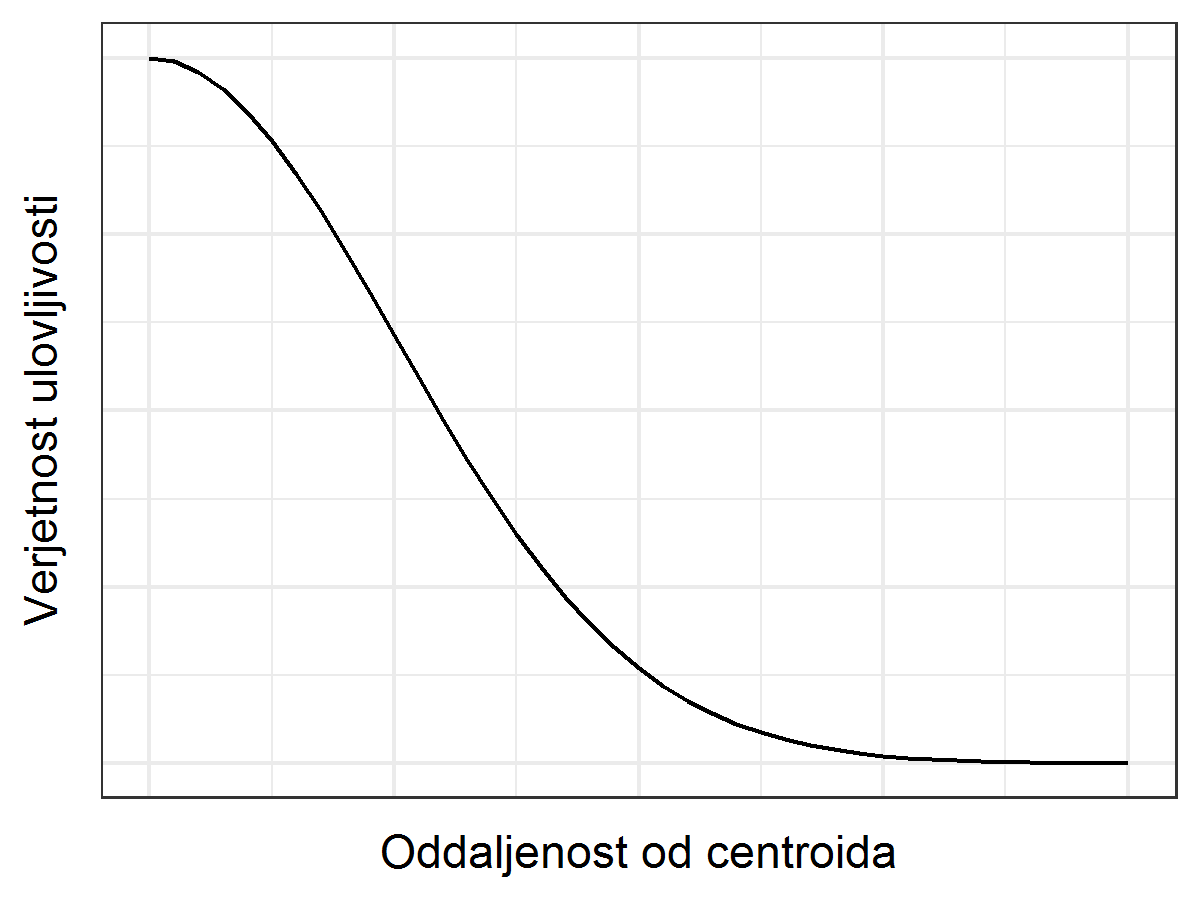
\includegraphics[width=0.5\linewidth]{../r_koda_slike/figures/half_normal.png}
  % \caption{A subfigure}
  \label{sli:sub2.1}
\end{subfigure}%
\begin{subfigure}{0.5\textwidth}
  \centering
  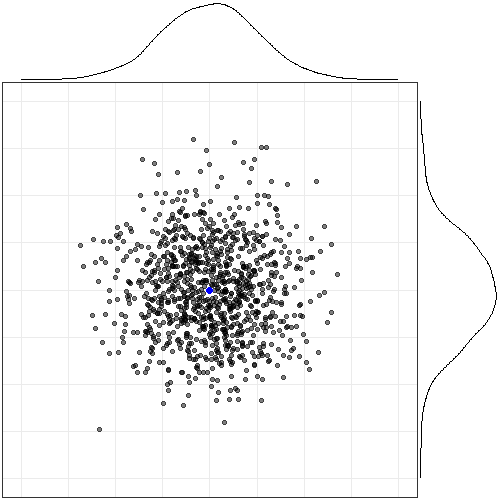
\includegraphics[width=0.5\linewidth]{../r_koda_slike/figures/homerange_usage.png}
  % \caption{A subfigure}
  \label{sli:sub2.2}
\end{subfigure}
\caption[Funkcija simuliranja vzorčnih točk]{Levo je ponazorjena verjetnost pojavljanja osebka oz. verjetnost, da ga zaznamo, v odvisnosti od oddaljenosti od centroida domačega okoliša. Prikaz desno ponazarja "ulov" osebka (sive pike) v prostoru, krivulje na desni in zgornji stranici pa sta robni gostoti.}
\label{sli:slika2}
\end{figure}

Osebkom, ki imajo pretežni delež domačega okoliša znotraj vzorčenega območja, lahko pripišemo delež njihovega domačega okoliša znotraj območja vzorčenja 1. V kolikor pa se centroid osebka nahaja v bližini roba območja vzorčenja, lahko pričakujemo, da bo del časa osebek preživel zunaj območja. V tem času med vzorčenjem ne bo zaznaven (ulovljiv), zato bo delež njegovega domačega okoliša znotraj območja vzorčenja manjši od 1. Podobno velja za krivulje, ki nimajo parametrične oblike (neparametrične krivulje).

Osebke med premikanjem lovimo in beležimo lokacijo in čas, ko smo jih zaznali. Točke na sliki \ref{sli:slika2} desno predstavljajo take ulove. Predpostavljamo, da te točke predstavljajo reprezentativno gibanje osebkov. Histogram razdalj med pari točk predstavlja razdalje, ki jih osebek lahko prehodi. To porazdelitev uporabimo pri izračunu deleža, ki pripada znotraj območja vzorčenja. Delež porazdelitve znotraj območja vzorčenja uporabimo v modelu kot individualno spremenljivko.

\subsubsection{Simulacije kot orodje za raziskovanje}
V matematičnih modelih opišemo pojav s funkcijami, ki so lahko preproste ali kompleksne. S kompleksnostjo pojava pa narašča tudi kompleksnost funkcij. Drug pristop je opis pojava s stohastičnimi procesi - simulacijami. Pojav razdelimo na manjše podenote in vsako enoto simuliramo kot samostojni proces. Razpon vrednosti, ki jih zavzemajo parametri podenote določi raziskovalec, najpogosteje na podlagi teoretskih osnov in poznavanje pojava. Podenota ni samostojna ampak je odvisna od drugih podenot in parametrov, ki jih določi raziskovalec. Primer take podenote je molekula vode, ki se obnaša na svoj način v razmerju do sosednjih molekul. Ko na sistem pogledamo od daleč lahko vidimo kako se le-ta obnaša glede na različne vhodne parametre. Na ta način simulirajo npr. ladijske elise, letalska krila ipd. V ekologiji lahko na tak način simuliramo gibanje in obnašanje živali ter preučujemo interakcijo med osebki oz. višjimi enotami in okoljem \citep{bolker_ecological_2008}.

\subsection{Cilji disertacije}
Cilj disertacije je izboljšati računanje gostote populacij, kjer med vzorčenjem prihaja do kršitve predpostavke o zaprtosti populacij.

Na podlagi razdalj med vzorčenimi lokacijami osebkov v območju vzorčenja bomo ocenili delež, ki ga osebek prebije znotraj območja vzorčenja. To informacijo bomo vključili v model za zaprte populacije kot individualno spremenljivko.

Ker bomo v modelu, ki upošteva individualno spremenljivko, v modeliranje vključili več informacij pričakujemo, da bo boljši od tistega, kjer te spremenljivke ne bomo uporabili. Za boljši model bomo smatrali tistega, ki bo imel nižji kriterij AICc.

Z vključitvijo informacije o morebitnem prehajanju roba vzorčenega območja v model, bomo izboljšali oceno ulovljivosti, saj bomo v model vključili eno od pomembnih komponent, ki vplivajo na spremenjeno zaznavnost in posledično ulovljivost osebkov. Pričakujemo, da bo model, ki vključuje individualno spremenljivko, uspešno kompenziral za spremenjeno ulovljivost zaradi prehoda čez rob območja vzorčenja.

Izboljšana ocena gostote bo na račun boljšega poznavanja velikosti dejanskega prispevka območja osebkov v območje vzorčenja, saj bomo iz gibanja osebkov lahko razbrali kako so razporejeni v prostoru.

Manjše kršitve predpostavke zaprtosti populacije ne bi smele bistveno vplivati na pristranskost ocene gostote. Pričakujemo, da bo razlika med ocenjeno in dejansko gostoto odvisna od razmerja med površino domačega okoliša in površino vzorčenega območja.

\section{Materiali in metode}
V našem primeru bo osnovni gradnik simulacije osebek \citep{deangelis_individual-based_2014}. Posamezniki v teh modelih imajo lastnosti, ki so lahko povezane s prostorom in časom, fiziološke lastnosti ali pa so v povezavi z drugimi osebki iste ali druge vrste. Ker parametre določimo sami, imamo veliko kontrole nad naključnostjo (stohastične), kar je še posebej uporabno pri proučevanju vpliva variabilnosti na pojav, ki ga raziskujemo.

\subsection{Simuliranje gibanja osebkov}
Simulacijo smo postavili v svet A, ki je tako velik, da noben simuliran osebek, ki ni imel nezanemarljivo možnost biti zaznan, ne bo imel praktične možnosti, da bi dosegel rob. To je delovalo kot varovalka, da ni prišlo do popačenja rezultatov pri simulacijah s parametri na skrajnosti svojih razponov. Znotraj sveta A smo centroide osebkov v območju S razporedili naključno s pomočjo enakomerne porazdelitve. Gibanje osebkov smo opisali z dvorazsežnostno normalno porazdelitvijo. V simulacijah smo generirali 500, 1000, 1500 in 2000 osebkov.

Polmer domačega okoliša osebkov smo določili v enotah standardnega odlkona ($\sigma$) normalne porazdelitve. V centroidu je imel osebek največjo ulovljivost, z oddaljenostjo od centroida pa verjetnost pada glede na funkcijo normalne porazdelitve.

\subsubsection{Odlov}
Osebke smo vzorčili s ponavljanjem v K odlovnih presledkih (5, 10, 15), kjer smo v posameznem presledku zabeležili po eno lokacijo na osebek. Ulovljivost je za vse osebke enaka in določena s parametrom $p$. Parameter $p$ smo simulirali med 0.1 in 0.3, kar predstavlja pogoste realne ulovljivosti, ki jih poročajo v študijah ulova-ponovnega ulova (npr. \citet{wilson_evaluation_1985, foster_critique_2012, chandler_characterizing_2018}).

Pri ulovu smo zabeležili tudi lokacijo znotraj vzorčenega območja, točke zabeležene zunaj pa smo krnili. Za osebke, od katerih smo dobili dva ali več vzorcev, smo izračunali vse možne pare razdalj med točkami. Te razdalje so osnova za izračun individualne spremenljivke.

\subsubsection{Izračun individualne spremenljivke}
Izračune smo izvajali na mreži celic oziroma rastru. Velikost celic smo nastavili na tako velikost, da po našem mnenju izbira velikosti ni vplivala na izračun. Glede na oddaljenost celice od centroida osebka smo s pomočjo posamezne funkcije za vsako celico rastra izračunali verjetnost pojavljanja, celice znotraj območja vzorčenja pa sešteli. Ta vrednost je povezana s časom, ki ga osebek porabi znotraj območja vzorčenja oziroma s časom, v katerem je na voljo za odlov.

\subsubsubsection{Dvorazsežnostna normalna porazdelitev}
Gibanje na podlagi dvorazsežnostne normalne porazdelitve se ujema s tistim, ki smo ga uporabili za simuliranje osebkov. Centroid smo izračunali kot geometrično sredino vseh vzorčenih točk osebka, za standardni odklon pa smo uporabili simulirano vrednost.

\subsubsubsection{Empirična porazdelitev}
Za prileganje empirične porazdelitve smo uporabili podatke o razdaljah med pari vseh možnih vzorčenih točk. Na podlagi števila celic in razdalje med centroidom vzorčenega območja in njegovim robom smo ustvarili primerno število razdelkov, katerih število ni vplivalo na točnost izračuna individualne spremenljivke. Vsako parno razdaljo smo uvrstili v razdelek in tako pridobili kumulativno število prehojenih razdalj (padajoča funkcija).

Razdelke smo dodatno utežili na sledeč način. V območje vzorčenja smo na podlagi enakomerne porazdelitve ustvarili toliko naključnih točk, kot je bilo vzorčenih parnih razdalj. Iz vseh empiričnih prehojenih razdalj smo s ponavljanjem vzorčili dolžine in jih postavili v prostor z izhodiščem v prej naključno vzorčenih točkah, smer daljice pa je bila naključna. Delež daljic, ki se je nahajal popolnoma znotraj območja vzorčenja, so predstavljali utež razreda. Uteženemu histogramu smo prilegli in ocenili funkcijo s tremi parametri, ki spominja na kumulativno porazdelitveno funkcije Weibullove porazdelitve.

\[
f(x) = e^{-(\frac{x}{\lambda})^{-k}}  \cdot a
\]

za $x >= 0$. Za lažji izračun deleža domačega okoliša znotraj vzorčenega območja smo dodali parameter $a$, ki spremeni vrednost, kjer funkcija seka $y$ os pri $x = 0$.
Za vse osebke smo predpostavili enako krivuljo, ki opiše rabo domačega okoliša okoli centroida. Na podlagi krivulje in območja vzorčenja smo izračunali relativni delež, ki ga posamezen osebek prebije znotraj vzorčenega območja.

Porazdelitev smo izbrali po tem, ko smo izkustveno določili, da relativno dobro opiše porazdelitev uteženih dolžine prehojenih razdalj.

\subsection{Ocenjevanje velikosti populacij}
Velikost populacije smo ocenili s pomočjo dveh modelov, Hugginsovega modela in modela CAPWIRE. Iz prvega smo izluščili parametra ulovljivost in velikost ocenjene populacije ter pripadajoče intervale zaupanja, iz drugega pa samo velikost populacije in pripadajoč interval zaupanja. V vseh primerih smo uporabili 95 \% interval zaupanja.

\subsubsection{Hugginsov model}
Z vzorčenjem smo za vsak osebek ustvarili odlovno zgodovino z individualno spremenljivko v K odlovnih presledkih. Delež časa, ki ga je osebek preživel znotraj območja vzorčenja glede na eno od zgoraj opisanih krivulj, smo uporabili kot individualno spremenljivko.

$M_0$: V prvem modelu smo predpostavili, da sta parametra za prvi in vsak nadaljnji ulov enaka ($c = p$), ulovljivost pa je odvisna samo od odlovne zgodovine (brez drugih spremenljivk). Ta model bi v zapisu, ki ga uporabljajo \citep{otis_statistical_1978}, imenovali $M_0$ in predpostavlja, da učinka roba ni.

$M_{sp}$: Za drugi model smo prav tako predpostavili enakost parametrov ($c = p$), ulovljivost pa je odvisna od individualne spremenljivke. Le-to smo izračunali na dva različna načina (glej poglavje Izračun individualne spremenljivke). Ta model bo predvidoma upošteval, da obstaja učinek roba in ga v nadaljevanju označujemo kot $M_{sp}$.

\subsubsection{Po modelu CAPWIRE}
Pri modeliranju s paketom CAPWIRE smo uporabili model TIRM, ki predpostavili, da gre za dve skupini osebkov z različnimi verjetnostmi ulovljivosti. Odlovne zgodovine smo sešteli po osebku in število ulovov uporabili v modelu.

\subsection{Statistike za primerjavo učinkovitosti delovanja popravka}
Za vsak set parametrov (npr. velikost populacije, velikost domačega okoliša, ulovljivost...) smo izračunali tri modele - po Hugginsovem modelu z in brez modifikacije ulovljivosti s pomočjo individualne spremenljivke ($M_0$, $M_{sp}$) in po modelu TIRM, kjer smo predpostavili dve skupini, ki imata lahko različni ulovljivosti.

Za vsak model smo zabeležili vrednosti parametrov, ki smo jih uporabili za simuliranje osebkov; število simuliranih osebkov, število odlovnih presledkov, polmer vzorčenega območja, število osebkov, ki smo jih zaznali (ujeli znotraj območja vzorčenja vsaj enkrat), standardni odklon uporabljen pri simuliranju domačega okoliša osebka, povprečni najdaljši premik in simulirana verjetnost ulovljivosti.

Od ocenjenih parametrov Hugginsovih modelov smo zabeležili oceno ulovljivosti za posamezen odlovni presledek (in pripadajoč 95\% interval zaupanja) za modela $M_0$ in $M_{sp}$, ocenjena velikost populacije (in pripadajoč 95\% interval zaupanja), AIC ter razliko v AIC med modeloma $M_0$ in $M_{sp}$. Za model TIRM smo shranili le velikost populacije in interval zaupanja, ker ocena ulovljivosti s Hugginsovim modelom ni neposredno primerljiva.
Poleg populacijskih statistik, ki jih je izračunal program MARK, smo shranili tudi parametre prileganja funkcij, s pomočjo katerih smo opisali parne razdalje med vzorčenimi točkami osebkov. Za (pol)normalno porazdelitev je to standardni odklon ($\sigma$), za empirično porazdelitev pa trije parametri ($\lambda$, $k$, $a$).

Za vsako simulacijo smo izračunali sledeče statistike:

\begin{itemize}
  \item Gostoto osebkov brez popravka, t.i. "naivna gostota". Izračunali smo jo z deljenjem števila simuliranih osebkov ($N$) z velikostjo območja vzorčenja.
  \item Gostoto osebkov s popravki, kjer smo vzorčeno območje povečali za razdaljo enako 50., 60., 70., 80., 90., 95. in 99. percentilu normalne ali empirične porazdelitve. Računanje percentila za normalno porazdelitev z znanim povprečjem in standardni odklon je preprosto. S pomočjo kvantilne funkcije (\emph{qnorm}) izračunamo pri kateri verjetnosti (prehojeni razdalji) je vrednost naključne spremenljivke manjša ali enaka dani verjetnosti.
  Za empirično porazdelitev kvantilna funkcija ni znana, oz. je relativno zapletena. S pomočjo simulacijskega pristopa in vzorčenjem z zavračanjem smo simulirali mnogo vrednosti, ki se prilegajo empirični porazdelitvi z znanimi parametri. Percentile smo izračunali na podlagi simuliranih vrednostih. Percentile smo uporabili kot razdaljo, za katero povesmo povečali čamo območje vzorčenja in posledično izračunali spremenjeno gostoto.
  \item AICc. Modela $M_0$ in $M_{sp}$, ki ocenita velikost populacije brez in s popravkom, smo primerjali glede na kriterij AICc. Kriterij nam omogoča rangirati modela, pri tem pa tehta med zapletenostjo in prileganjem modela podatkom. Uporabili bomo AICc, ki se od AIC razlikuje po tem, da je bolj primeren za manjše vzorce. Model z nižjo vrednostjo AICc in za razliko vsaj 2, bo boljši od drugega modela.
\end{itemize}

Izračunane statistike gostote smo primerjali s pravo gostoto, t.i. zlatim standardom, ki smo ga izračunali tako, da smo število generiranih centroidov (osebkov) delili s površino, ki smo jo uporabili za generiranje teh osebkov. Izračunali smo kazalnik, ki prikazuje delež ocenjene gostote od prave gostote ($I = \frac{\hat{D}}{D}$).

Za prikaz trendov in razlik med skupinami smo uporabili posplošen linearnen model (t.i. GLM, \citet{faraway_extending_2006}), z normalno razporejenimi ostanki.

Simulacije smo spisali v programskem okolju \Q{R} \citep{r_core_team_r_2018}. Pri tem bomo uporabili pakete \Q{sp} \citep{bivand_applied_2008}, \Q{raster} \citep{hijmans_ability_2006}, \Q{rgeos} \citep{bivand_rundel_2017}, \Q{cluster} \citep{maechler_et_al_2018}, \Q{splancs} \citep{rowlingson_diggle_2017}, \Q{foreach} \citep{microsoft_2017}) in \Q{doParallel} \citep{doparallel_2017}.

Za oceno parametrov Hugginsovega modela smo uporabili paket \Q{RMark} \citep{laake_2013}, ki omogoča posredno povezavo s programom \Q{MARK} \citep{cooch_program_2012}. Model \Q{TIRM} smo ocenili s pomočjo \Q{R} paketa \Q{capwire} \citep{pennell_miller_2012}. Za vse grafike smo uporabili paket \Q{ggplot2} \citep{wickham_ggplot2_2009}.

Simulacije bomo poganjali na delovni postaji na Oddelku za biologijo Katedra za ekologijo in varstvo okolja. Postaja ima v dveh procesorjih 24 sredic in 48 niti ter več kot 100 GB delovnega spomina. Osnovni operacijski sistem je CentOS, v katerem tečejo virtualni sistemi (odprtokodni sistemu Ubuntu 18.04). Disertacija je bila oblikovana s sistemom \LaTeX.

\section{Rezultati}

\subsection{Simulacije}
Skupno smo izvedli 6000 simulacij. Tri tisoč simulacij smo izvedli na način, da smo individualno spremenljivko izračunali s pomočjo simuliranih vrednosti standardnega odklona (normalna porazdelitev) in na podlagi vzorčenih točk izračunanim centroidom kot povprečje ($\mu$). S pomočjo programa MARK smo uspešno ocenili v 2916 simulacijah.
Enako število simulacij smo izvedli za primer, kjer smo krivuljo za izračun individualne spremenljivke ocenili iz podatkov (empirična porazdelitev). Pri oceni parametrov smo bili uspešni 2681-krat (Tabela \ref{tab:tabela1}).

Da nekaterih modelov nismo uspešno ocenili je po pričakovanjih. Zaradi določene strukture podatkov je možno, da optimizacijski kriterij znotraj parametrskega prostora ne najde optimuma, ali pa so ocenjeni parametri na intervalu $- \infty < x < \infty$. Tiste simulacije, ki niso dale smiselnega rezultata, smo iz analize izključili.

Na polno obremenjenem računalniku je bila simulacija izračuna individualne spremenljivke končana v približno 48 urah. Nadaljnje analize ulova in ponovnega ulova ter priprava podatkov za analizo pa so zahtevale še dodatnih šest ur.

Zaznati je mogoče vzorec v številu uspešnih simulacij glede na uporabljeno funkcijo. Število uspešnih simulacij glede na število generiranih osebkov in število odlovnih intervalov se med tema dvema skupinama razlikuje. Večina neuspelih simulacij pri uporabi empirične funkcije je za najmanjše število odlovnih intervalov ($K=5$).

\begin{table}[!htb]
  \caption{Prikaz števila simulacij, kjer smo uspešno ocenili parametre, glede na funkcijo, ki je bila uporabljena za izračun individualne spremenljivke. V vrsticah je število generiranih osebkov ($N$), v stolpcih pa število odlovnih intervalov ($K$). Uspešno izračunanih simulacij z empirično funkcijo je nekoliko manj. Za lažjo predstavo v spodnji matriki prikazujemo razliko med zgornjima tabelama tako, da smo empirični (levo) odšteli normalno (desno) tabelo. Pretežni delež neuspelih simulacij je predvsem na račun simulacij, ki imajo 5 odlovnih intervalov in/ali manjše število simuliranih osebkov (nižja gostota).}
  \label{tab:tabela1}
\begin{tabular}{cc}
    \begin{minipage}{.33\linewidth}
      \caption*{Empirična funkcija}
      \resizebox{\columnwidth}{!}{%
        \begin{tabular}{rccc}
          \toprule
           & \textbf{$K=5$} & \textbf{$k=10$} & \textbf{$K=15$} \\
          \midrule
          $N=500$ & 142 & 187 & 190 \\
          $N=800$ & 141 & 192 & 178 \\
          $N=1000$ & 135 & 182 & 185 \\
          $N=1300$ & 168 & 212 & 194 \\
          $N=1500$ & 171 & 186 & 218 \\
          \bottomrule
        \end{tabular}
        }
    \end{minipage}%

    \begin{minipage}{.33\linewidth}
      \caption*{Normalna funkcija}
      \resizebox{\columnwidth}{!}{%
        \begin{tabular}{rccc}
          \toprule
           & \textbf{$K=5$} & \textbf{$k=10$} & \textbf{$K=15$} \\
          \midrule
          $N=500$ & 188 & 209 & 197 \\
          $N=800$ & 179 & 205 & 183 \\
          $N=1000$ & 175 & 190 & 185 \\
          $N=1300$ & 191 & 212 & 195 \\
          $N=1500$ & 199 & 190 & 218 \\
          \bottomrule
        \end{tabular}
        }
    \end{minipage}%

    \begin{minipage}{.33\linewidth}
      \caption*{Razlike med matrikama}
      \resizebox{\columnwidth}{!}{%
        \begin{tabular}{rccc}
          \toprule
           & \textbf{$K=5$} & \textbf{$k=10$} & \textbf{$K=15$} \\
          \midrule
          $N=500$ & -46 & -22 & -7 \\
          $N=800$ & -38 & -13 & -5 \\
          $N=1000$ & -40 & -8 & 0 \\
          $N=1300$ & -23 & 0 & -1 \\
          $N=1500$ & -28 & -4 & 0 \\
          \bottomrule
        \end{tabular}
        }
    \end{minipage}
\end{tabular}
\end{table}

\subsection{Parameter p modelov $M_0$ in $M_{sp}$ po Hugginsu}
Za modela $M_0$ in Msp modelu smo predpostavili, da sta parametra $p$ in $c$ enaka. Ulovljivost v prvem in vseh ostalih odlovnih presledkih predpostavljamo enako. Zato v analizi obravnavamo le parameter ulovljivosti $p$. Za lažjo primerjavo smo izračunali razmerje med ocenjeno in simulirano vrednostjo $p$ (slika \ref{sli:slika3}). Model TIRM oceni $p$ za dve skupini, kar neposredno ni primerljivo s parametrom $p$ po Hugginsovem modelu, zato le-tega nismo podrobneje preučili.

V povprečju je ulovljivost za vse simulacije in modele podcenjena in je približno med 0.35 in 0.4 deleža simulirane vrednosti. Ulovljivost ocenjena po modelu Msp je nekoliko bolj podcenjena, ne glede na to s pomočjo katere porazdelitve izračunamo individualno spremenljivko. V povprečju je ulovljivost za primer empirične porazdelitve za oba modela nekoliko nižja (za približno 0.01). Vidimo tudi, da se razlika med modeloma rahlo zmanjša s povečanjem simulirane ulovljivosti (slika \ref{sli:slika3}).

\subsubsection{Primerjava simulirane in ocenjene ulovljivosti glede na porazdelitev}
\subsubsubsection{Empirična porazdelitev}
Povprečje deleža simulirane vrednosti preprostega $M_0$ modela je 0.397, modela z individualno spremenljivko $M_{sp}$ pa za 0.035 nižja.

\begin{verbatim}
Call:
glm(formula = p.val ~ p.var, data = xep)

Deviance Residuals:
 	Min    	1Q	Median    	3Q   	Max
-0.36868  -0.16667  -0.07254   0.09971   1.44373

Coefficients:
              	Estimate Std. Error t value Pr(>|t|)
(Intercept)   	0.397081   0.001467  270.69   <2e-16 ***
p.varp.target.sp -0.035010   0.002075  -16.88   <2e-16 ***
---
Signif. codes:  0 ‘***’ 0.001 ‘**’ 0.01 ‘*’ 0.05 ‘.’ 0.1 ‘ ’ 1

(Dispersion parameter for gaussian family taken to be 0.05769313)

	Null deviance: 3109.8  on 53619  degrees of freedom
Residual deviance: 3093.4  on 53618  degrees of freedom
AIC: -786.36
\end{verbatim}

\subsubsubsection{Normalna porazdelitev}
Povprečje deleža simulirane vrednosti preprostega $M_0$ modela je 0.387, modela z individualno spremenljivko $M_{sp}$ pa 0.349 (0.038 nižja).

\begin{verbatim}
Call:
glm(formula = p.val ~ p.var, data = xep)

Deviance Residuals:
 	Min    	1Q	Median    	3Q   	Max
-0.35876  -0.16239  -0.07163   0.09433   1.45364

Coefficients:
              	Estimate Std. Error t value Pr(>|t|)
(Intercept)   	0.387167   0.001381  280.29   <2e-16 ***
p.varp.target.sp -0.037886   0.001953  -19.39   <2e-16 ***
---
Signif. codes:  0 ‘***’ 0.001 ‘**’ 0.01 ‘*’ 0.05 ‘.’ 0.1 ‘ ’ 1

(Dispersion parameter for gaussian family taken to be 0.05563641)

	Null deviance: 3265.5  on 58319  degrees of freedom
Residual deviance: 3244.6  on 58318  degrees of freedom
AIC: -2972.7
\end{verbatim}

\begin{figure}[H]
\centering
\begin{subfigure}[b]{0.75\textwidth}
  \centering
  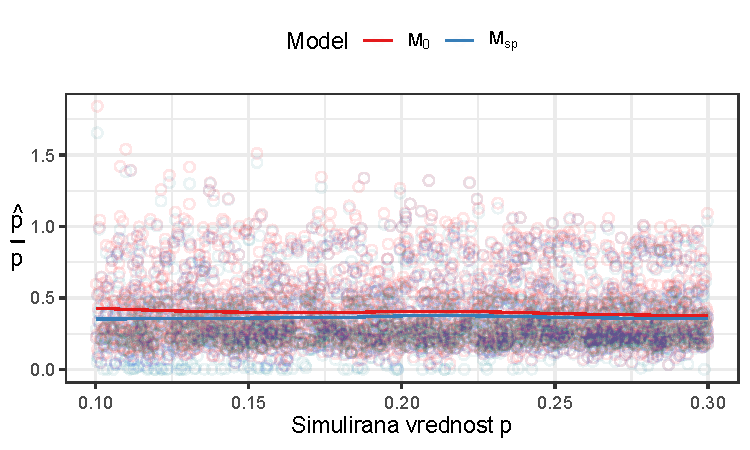
\includegraphics[width=1\linewidth]{C:/Users/romunov/Documents/workspace/doktorat/analiza/figures/E-0a_pristranskost_1_in_sp_ocene_ulovljivosti.pdf}
  \label{sli:sub3.1}
\end{subfigure}

\begin{subfigure}[b]{0.75\textwidth}
  \centering
  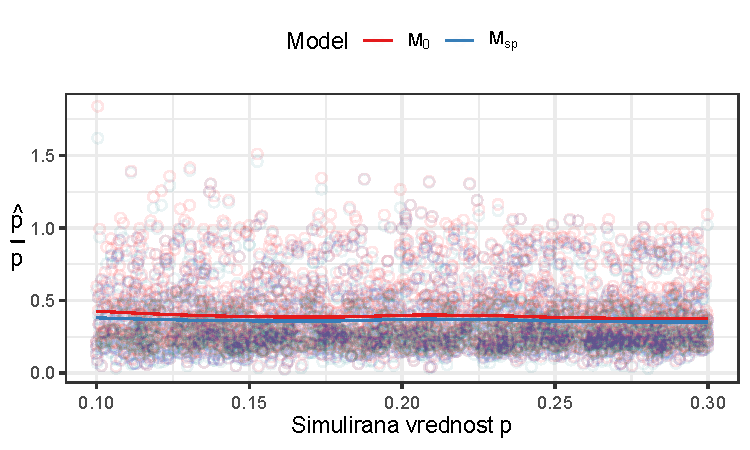
\includegraphics[width=1\linewidth]{C:/Users/romunov/Documents/workspace/doktorat/analiza/figures/N-0a_pristranskost_1_in_sp_ocene_ulovljivosti.pdf}
  \label{sli:sub3.2}
\end{subfigure}

\caption[Primerjava ocenjene ulovljivosti s simulirano]{Povprečna ocena ulovljivosti (parameter $p$) za Hugginsova modela $M_0$ in $M_{sp}$. Na osi $x$ so prikazane simulirane vrednosti $p$, na osi $y$ pa razmerje med ocenjeno in simulirano vrednostjo. V primeru, da ne bi bilo kršenih predpostavk, bi morala biti ocena in simulirana vrednost približno podobni (in njuno razmerje $\sim 1$). Izračun individualne spremenljivke s pomočjo empirične (zgoraj) in normalne funkcije (spodaj). Ne kaže, da izbira funkcije za izračun individualne spremenljivke bistveno vpliva na oceno parametra $p$.}
\label{sli:slika3}
\end{figure}

\subsubsection{Primerjava ulovljivosti glede na število simuliranih osebkov}
Ocena ulovljivosti ($p$) glede na število simuliranih osebkov kaže podobno sliko (slika \ref{sli:slika4}). V povprečju model, kjer smo uporabili za izračun še individualno spremenljivko ($M_{sp}$), bolj podcenjuje ulovljivost kot model brez nje ($M_0$). Ta razlika je relativno majhna.

Opazili smo tudi trend, da je razkorak med modeloma večji za simulacije z manj osebki za manjše simulirane ulovljivosti. Z večanjem simuliranega parametra p se razlika zmanjšuje tudi za primere z najmanjšim številom simuliranih osebkov. Razlike med simulacijami, kjer smo individualno spremenljivko izračunali s pomočjo empirične ali normalne porazdelitve, so relativno majhne.

\begin{figure}[H]
\centering
\begin{subfigure}[b]{1\textwidth}
  \centering
  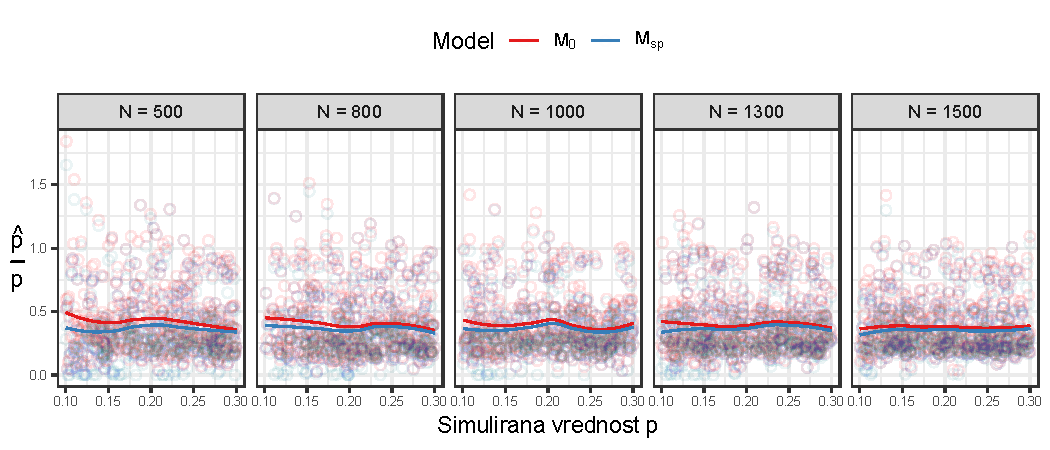
\includegraphics[width=1\linewidth]{C:/Users/romunov/Documents/workspace/doktorat/analiza/figures/E-0b_pristranskost_p1_in_psp_glede_na_st_walkerjev.pdf}

  \label{sli:sub4.1}
\end{subfigure}

\begin{subfigure}[b]{1\textwidth}
  \centering
  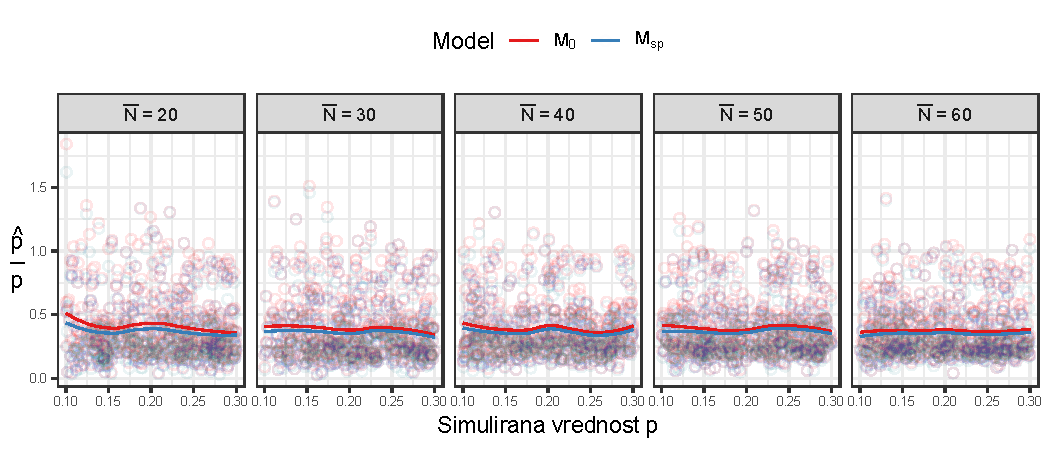
\includegraphics[width=1\linewidth]{C:/Users/romunov/Documents/workspace/doktorat/analiza/figures/N-0b_pristranskost_p1_in_psp_glede_na_st_walkerjev.pdf}
  \label{sli:sub4.2}
\end{subfigure}

\caption[Primerjava ocenjene ulovljivosti s simulirano glede na število simuliranih osebkov]{Zgornja slika prikazuje podatke, kjer smo individualno spremenljivko ocenili s pomočjo empirične spremenljivke, spodnja pa podatke za simulacije, kjer smo individualno spremenljivko izračunali s pomočjo normalne porazdelitve. Točke prikazujejo razmerje med oceno ulovljivosti in pravo, simulirano, vrednostjo glede na število generiranih osebkov. Na x osi so prikazane simulirane vrednosti ulovljivosti, na y osi pa razmerje med ocenjeno in simulirano vrednostjo. Okenca prikazujejo podatke glede na število simuliranih osebkov (od 500 do 1500).}
\label{sli:slika4}
\end{figure}

\subsubsection{Primerjava ulovljivosti glede na razmerje velikosti domačega okoliša in območja vzorčenja}
S slike \ref{sli:slika5} je razvidno, da je vpliv zelo velik. Ko je razmerje velikosti domačega okoliša in velikosti območja vzorčenja majhno (majhen domač okoliš v primerjavi z območjem zvorčenja), je ocena parametra relativno zanesljiva. Z večanjem razmerja med domačim okolišem in območjem vzorčenja pa se zanesljivost ocene poslabšuje in se celo spusti pod globalno povprečje.

Sodeč po naših rezultatih s slike \ref{sli:slika5}, ne moremo sklepati, da ima število generiranih osebkov v povezavi z razmerjem domačega okoliša in vzorčenega območja bistven vpliv na oceno ulovljivosti oz. je vpliv neznaten. Razlike med simulacijami, kjer smo spreminjali funkcijo za izračun individualne spremenljivke, so majhne oz. jih ni.

\begin{figure}[H]
\centering
\begin{subfigure}[b]{1\textwidth}
  \centering
  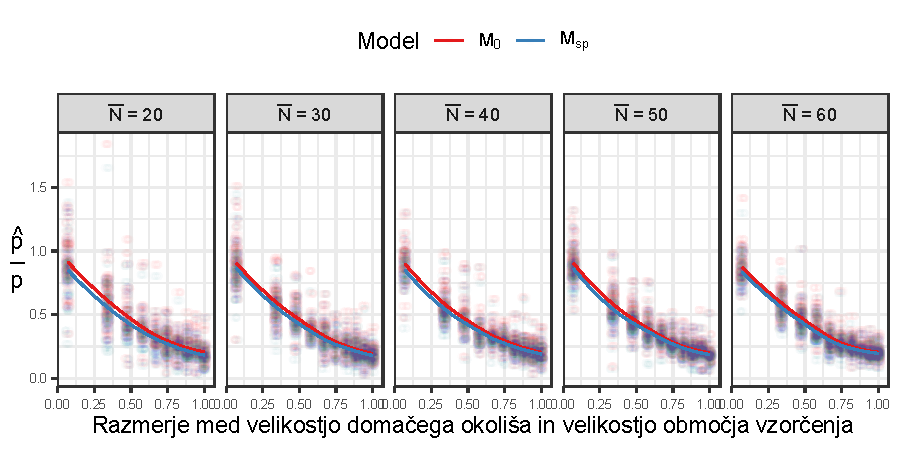
\includegraphics[width=1\linewidth]{C:/Users/romunov/Documents/workspace/doktorat/analiza/figures/E-0f_pristranskost_p_glede_na_sap_hr_ratio_po_st_gen_walkerjev_brez_popravka.pdf}

  \label{sli:sub5.1}
\end{subfigure}

\begin{subfigure}[b]{1\textwidth}
  \centering
  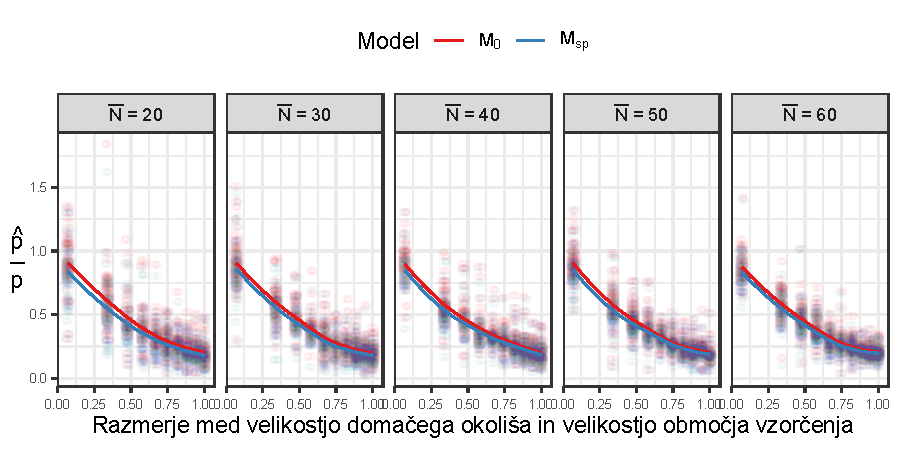
\includegraphics[width=1\linewidth]{C:/Users/romunov/Documents/workspace/doktorat/analiza/figures/N-0f_pristranskost_p_glede_na_sap_hr_ratio_po_st_gen_walkerjev_brez_popravka.pdf}
  \label{sli:sub5.2}
\end{subfigure}

\caption[Vpliv razmerja med ocenjeno in pravo ulovljivostjo v povezavi z razmerjem velikosti domačega okoliša in vzorčenega območja.]{Vpliv razmerja med ocenjeno in pravo ulovljivostjo v povezavi z razmerjem velikosti domačega okoliša in vzorčenega območja. Zgornja slika je za simulacije, kjer smo individualno spremenljivko izračunali s pomočjo empirične porazdelitve, spodnja pa s pomočjo normalne porazdelitve.}
\label{sli:slika5}
\end{figure}

Razmerje med površinama domačega okoliša in območja vzorčenja ima na pristranskost ocene parametra $p$ velik vpliv. Na sliki 6 je prikazano kako se pristranskost ocene parametra $p$ spreminja z razmerjem površin domačega okoliša in vzorčenega območja glede na število generiranih osebkov in odlovnih presledkov. Povprečji ocen obeh Hugginsovih modelov konvergirata z večanjem razmerja, kjer več simuliranih osebkov pomeni bolj podobno (in pristransko) oceno med modeloma. Podoben vpliv ima tudi število odlovnih presledkov, poleg tega pa le-ti vpliva tudi na variabilnost ocen. Več kot je odlovnih presledkov, manjša je variabilnost v oceni. S slike \ref{sli:slika6} ne moremo trditi, da smo zaznali bistvene razlike med simulacijami, kjer smo za izračun individualne spremenljivke uporabili normalno ali empirično funkcijo.

\begin{figure}[H]
\centering
\begin{subfigure}[b]{1\textwidth}
  \centering
  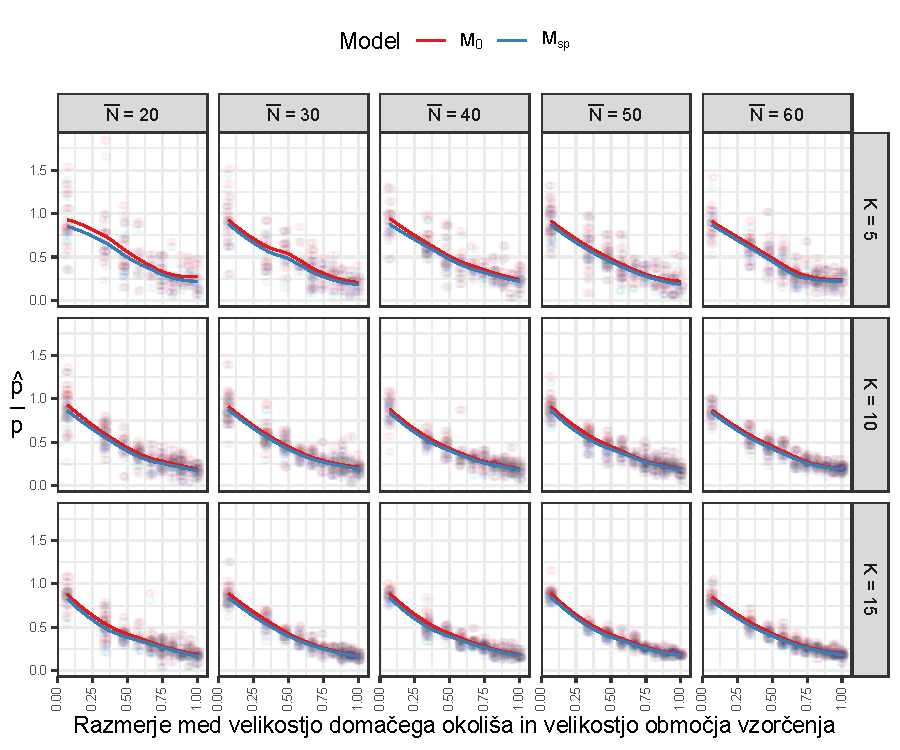
\includegraphics[width=0.8\linewidth]{C:/Users/romunov/Documents/workspace/doktorat/analiza/figures/E-0h_pristranskost_p_glede_sap_hr_razmerje_glede_na_st_walkerjev_in_st_sessionov.pdf}
  \label{sli:sub6.1}
\end{subfigure}

\begin{subfigure}[b]{1\textwidth}
  \centering
  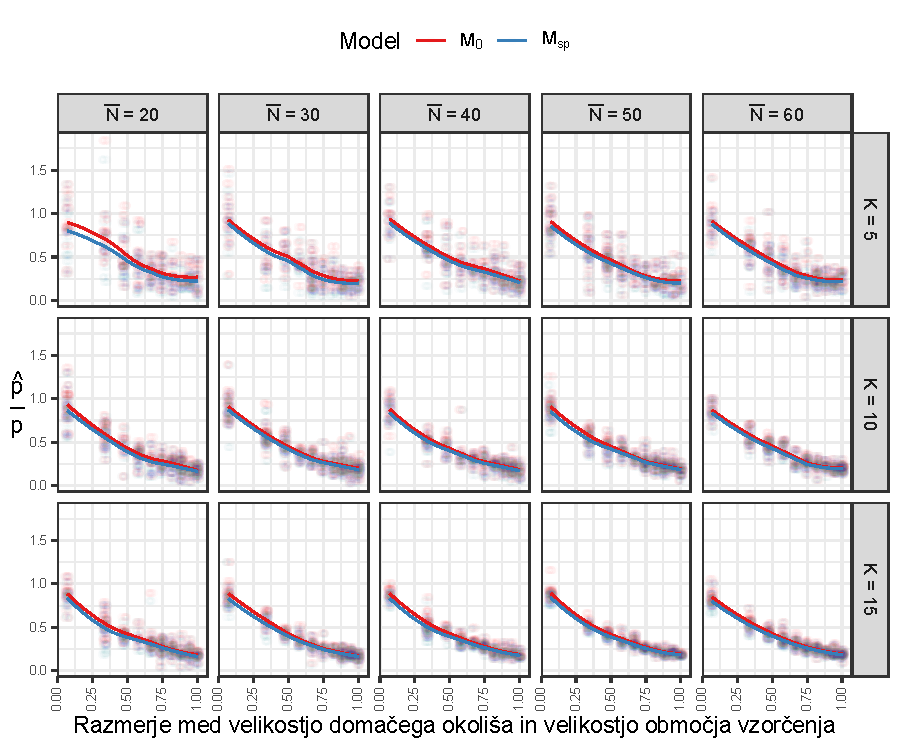
\includegraphics[width=0.8\linewidth]{C:/Users/romunov/Documents/workspace/doktorat/analiza/figures/N-0h_pristranskost_p_glede_sap_hr_razmerje_glede_na_st_walkerjev_in_st_sessionov.pdf}
  \label{sli:sub6.2}
\end{subfigure}
\caption[Prikaz pristranskosti ocene ulovljivosti ($p$) glede na razmerje površin domačega okoliša in območja vzorčenja v povezavi s številom simuliranih osebkov (stolpci) in odlovnih presledkov (vrstice).]{Prikaz pristranskosti ocene ulovljivosti ($p$) glede na razmerje površin domačega okoliša in območja vzorčenja v povezavi s številom simuliranih osebkov (stolpci) in odlovnih presledkov (vrstice). Na prvi sliki so prikazani rezultati simulacij, kjer smo za izračun individualne spremenljivke uporabili empirično, na spodnji pa normalno funkcijo. Na osi $x$ je prikazano razmerje od 0 (površina domačega okoliša zelo majhna v primerjavi s površino vzorčenega območja) do 1 (površina domačega okoliša in vzorčenega območja enako velika). Pristranskost ocene parametra $p$ narašča z večanjem razmerja velikosti domačega okoliša in območja vzorčenja. Povprečja ulovljivosti modelov po Hugginsu konvergirajo. Z večanjem števila simuliranih osebkov se manjša tudi razlika v oceni parametra. Podobno sliko vidimo z večanjem števila odlovnih presledkov (vrstice), kjer poleg konvergence povprečij modelov opazimo tudi manjšanje variance ocene.}
\label{sli:slika6}
\end{figure}

\subsection{Gostota}
Dejansko gostoto smo izračunali kot število centroidov (osebkov) znotraj površine, kjer smo jih simulirali. S pomočjo modelov Huggins in TIRM smo dobili oceno številčnosti znotraj območja vzorčenja. Ker so osebki hodili čez mejo vzorčenega območja, smo tako dejansko ocenili velikost superpopulacije katere prostorska omejenost ni nedvoumno določena. Na podlagi ocenjenega števila osebkov in velikosti vzorčenega območja smo izračunali gostoto te superpopulacije. Za izračun gostote smo uporabili tudi razširjeno območje vzorčenja. Območje smo razširili tako, da smo polmer povečali za določeno razdaljo. Razdaljo smo izbrali kot percentil parne razdalje iz funkcije, ki smo jo ali prilegli podatkom (empirična funkcija) ali pa izračunali na podlagi simuliranih parametrov (dvorazsežna normalna porazdelitev). Gostoto smo izračunali glede na območje povečano za standardni odklon polmera simuliranega območja gibanja osebka (hr), za percentil porazdelitve (50-99) oz. za najdaljšo prehojeno razdaljo (effect) v posamezni simulaciji. Spodnji rezultati so podani kot razmerje med ocenjeno in pravo gostoto. Ker gre za razmerje kjer je prava gostota v imenovalcu, se bodo v primeru nepristransko ocenjene gostote vrednosti nahajale blizu 1.

\subsubsection{Razlike v gostoti glede na število simuliranih osebkov in funkcij za izračun individualne spremenljivke}
Na sliki \ref{sli:slika6} so prikazani podatki izračuni gostot. Na sliki uporabimo kazalnik, ki je z gostoto povezan kot razmerje med gostoto izračunano iz ocenjene velikosti populacije in simulirane velikosti populacije ($\hat{D}/D$).

Opazimo razlike med simulacijami, kjer smo uporabili empirično in normalno porazdelitev za izračun individualne spremenljivke. Razlike so predvsem v primerih, kjer smo območje vzorčenja povečani za razdaljo od 50. do 99. percentila. Pristranskost kazalnika se v odvisnosti od razmerja domačega okoliša in vzorčenega območja povečuje hitreje za primere, ko smo za izračun individualne spremenljivke uporabili empirično porazdelitev.

Pristranskost kazalnika v primeru nepovečanega območje hitro narašča z večanjem razmerja med velikostjo domačega okoliša in velikostjo območja vzorčenja podobno za oba načina izračuna individualne spremenljivke.

Z manjšanjem razmerja med površino domačega okoliša in območja vzorčenja se pristranskost v povprečju zmanjšuje. Za primere, kjer smo za izračun individualne spremenljivke uporabili empirično funkcijo, je gladilka za večja povečanja razmerja bolj konkavne oblike, s povečevanjem površine vzorčenega območja za izračun gostote pa se pristranskost v splošnem zmanjšuje.

Pri simulacijah, kjer smo za izračun individualne spremenljivke uporabili normalno porazdelitev je konkavnosti  možno opaziti le za primere, kjer smo območje vzorčenja povečali za najdaljšo prehojeno razdaljo (zadnji stolpec).
Za oba načina izračuna individualnih spremenljivk pa velja, da se povečanje površine vzorčenega območja pozna najmanj za tiste simulacije, kjer je bilo razmerje med velikostjo domačega okoliša in velikostjo vzorčenega območja najmanjše.

Povečevanje števila simuliranih osebkov prispeva predvsem k zmanjšanju variabilnosti ocen velikosti populacij in posledično k manjši variabilnosti gostot. Variabilnost je za veliko večino primerov najmanjša za simulacije, kjer je razmerje med velikostjo domačega okoliša in velikostjo vzorčenega območja najmanjša.

Razlike med modeli so med scenariji primerljivi. Najbolj precenjene rezultate da model TIRM, manj $M_{sp}$ in najmanj $M_0$. Razlike med modeli izginejo predvsem na račun povečanja razmerja med površinama domačega okoliša in območja vzorčenja.

\begin{figure}[H]
  \centering
  \begin{subfigure}[b]{1\textwidth}
    \centering
    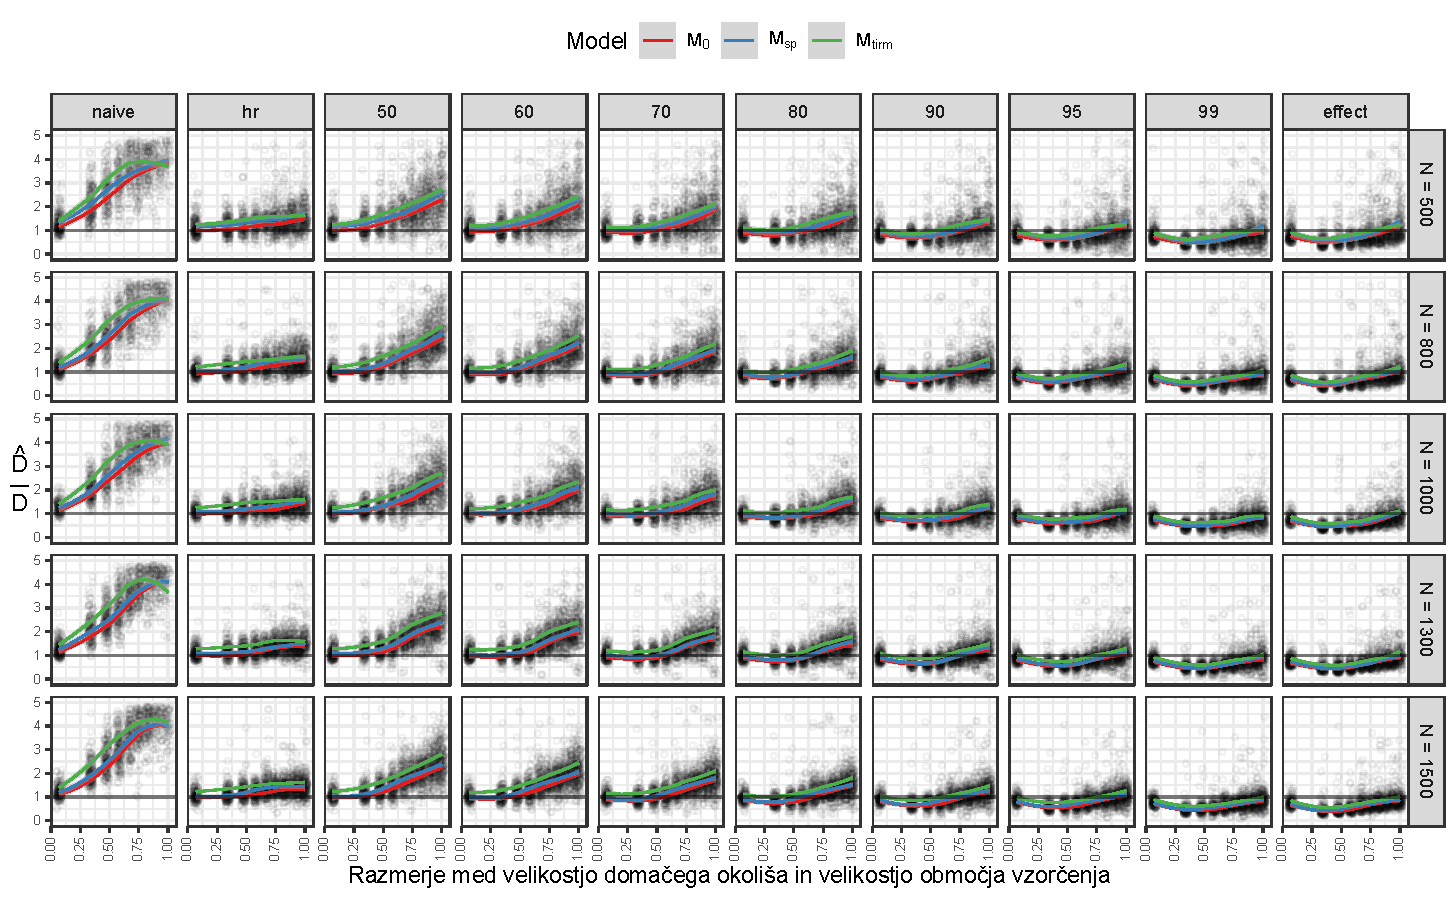
\includegraphics[width=1\linewidth]{C:/Users/romunov/Documents/workspace/doktorat/analiza/figures/E-1a_gostota_gled_na_razmerje_hr_sap_po_correction_type_in_st_gen_walk.pdf}
    \label{sli:sub7.1}
  \end{subfigure}

  \begin{subfigure}[b]{1\textwidth}
    \centering
    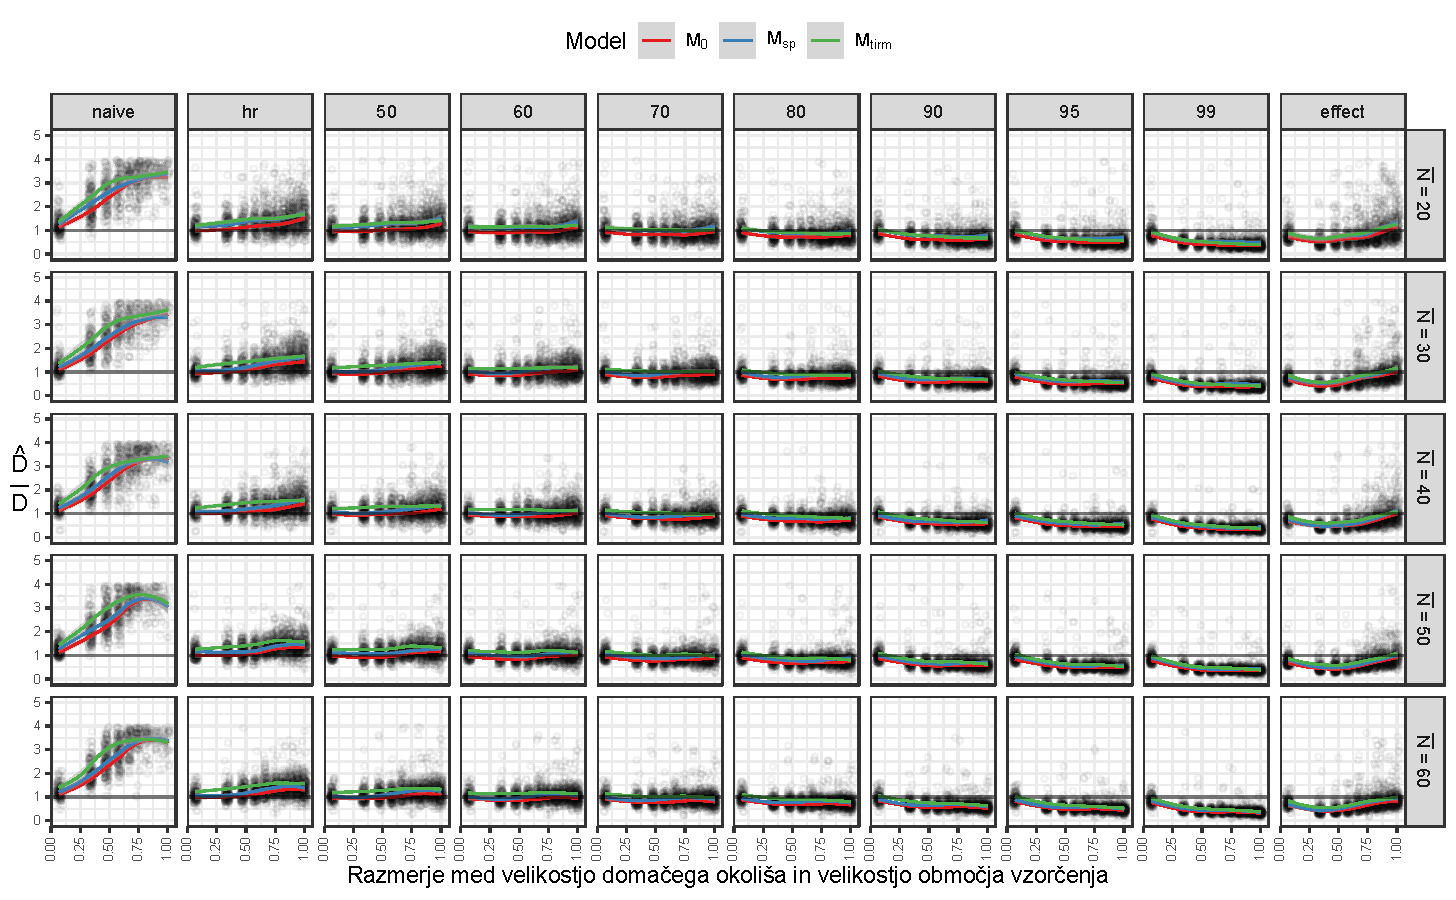
\includegraphics[width=1\linewidth]{C:/Users/romunov/Documents/workspace/doktorat/analiza/figures/N-1a_gostota_gled_na_razmerje_hr_sap_po_correction_type_in_st_gen_walk.pdf}
    \label{sli:sub7.2}
  \end{subfigure}
  \caption[Prikaz kazalnika gostot ($\hat{D}/D$)]{Prikaz kazalnika gostot ($\hat{D}/D$). Na zgornji sliki so prikazani rezultati za simulacije, kjer smo za izračun individualne spremenljivke uporabili empirično porazdelitev, na spodnji pa dvorazsežno normalno porazdelitev. Stolpci oken ponazarjajo razširitev vzorčenega območja za percentil dane porazdelitve, vrstice pa število simuliranih osebkov, na podlagi katerih smo izvedli vzorčenje in posledično izračun velikosti populacije in gostote. Pri izračunu smo uporabili tri modele, Hugginsov model $H_0$, $H_{sp}$, kjer smo ulovljivost modelirali glede na individualno spremenljivko in TIRM, ki predpostavlja dve skupini z različno ulovljivostjo.}
  \label{sli:slika7}
\end{figure}

\subsubsection{Razlike v gostoti glede na funkcijo za izračun individualne spremenljivke, števila odlovnih intervalov ter število simuliranih osebkov}
Na slikah \ref{sli:slika7} in \ref{sli:slika8} smo podatke s slike \ref{sli:slika6} prikazali tako, da so podatki razdeljeni na odlovne presledke ($K = [5, 10, 15]$). Pogled glede na število odlovnih presledkov nam je dal predvsem vpogled v spremembo variabilnosti. Pri simulacijah z najnižjim $K$ ($K = 5$) je varianca večja kot pri tistih s $K = [10, 15]$. Pri slednjih že opazimo prevladujoč vzorec v povprečju kazalnika za vse modele glede na popravke velikosti območja vzorčenja (stolpci) in število simuliranih osebkov (vrstice). Vpliv povečanja površine vzorčenega območja se opazi predvsem za simulacije, kjer je razmerje med velikostjo domačega okoliša in velikostjo vzorčenega območja relativno velika. Na simulacije, kjer je to razmerje relativno majhno, povečanje območja vzorčenja pri pristranskosti ne kaže očitnega učinka.

\begin{figure}[H]
  \centering
  \begin{subfigure}[b]{1\textwidth}
    \centering
    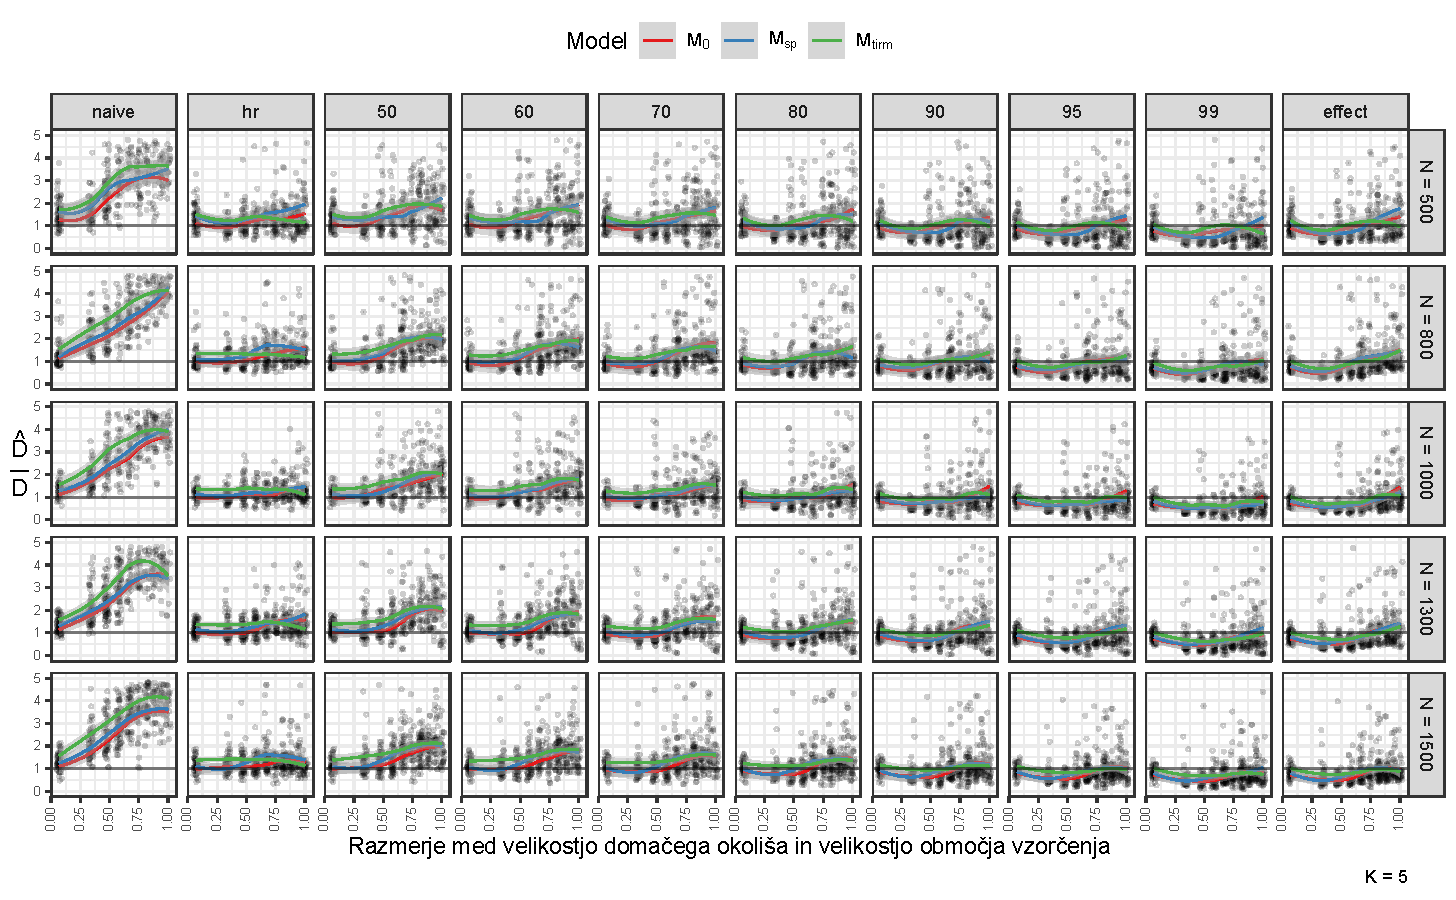
\includegraphics[width=1\linewidth]{C:/Users/romunov/Documents/workspace/doktorat/analiza/figures/E-1c_gostota_gled_na_razmerje_hr_sap_po_correction_type_in_st_gen_walk_za_k5.pdf}
    \label{sli:sub8.1}
  \end{subfigure}

  \begin{subfigure}[b]{1\textwidth}
    \centering
    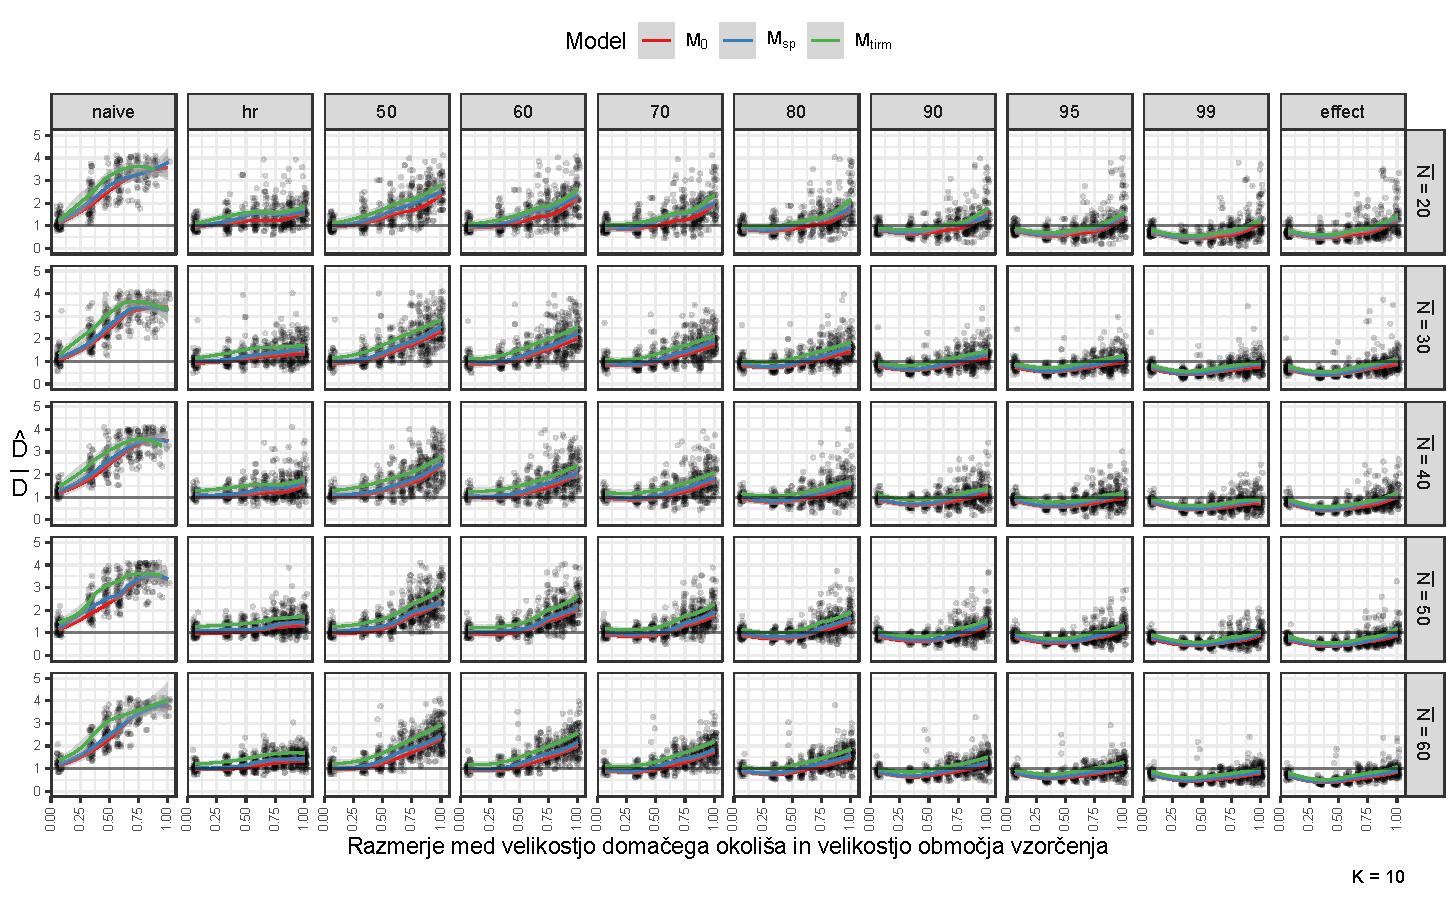
\includegraphics[width=1\linewidth]{C:/Users/romunov/Documents/workspace/doktorat/analiza/figures/E-1d_gostota_glede_na_razmerje_hr_sap_po_correction_type_in_st_gen_walk_za_k10.pdf}
    \label{sli:sub8.2}
  \end{subfigure}
\end{figure}

\begin{figure}[H]
  \ContinuedFloat
  \begin{subfigure}[b]{1\textwidth}
    \centering
    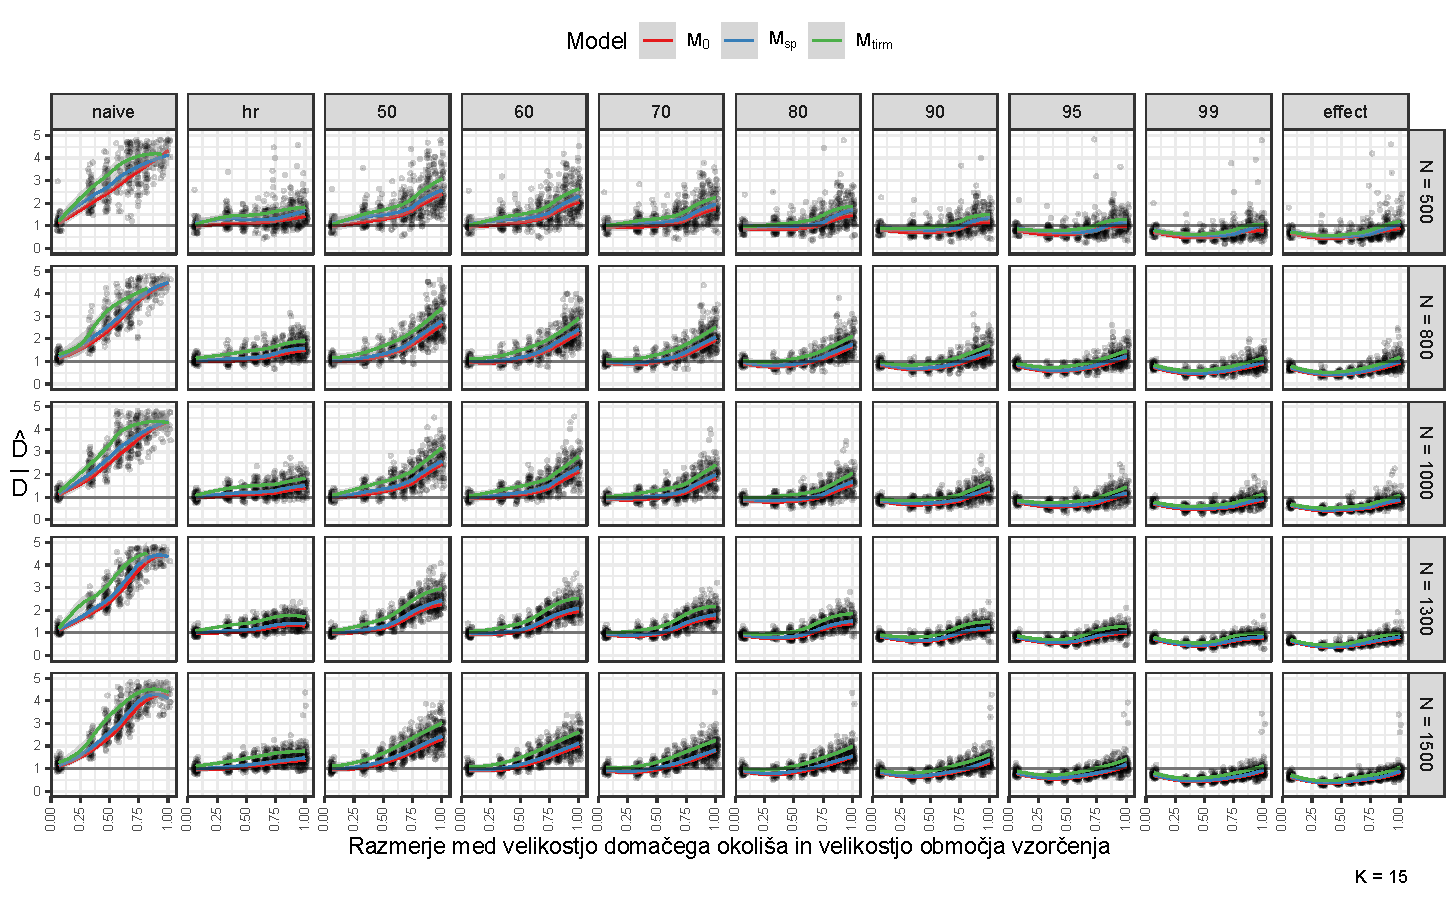
\includegraphics[width=1\linewidth]{C:/Users/romunov/Documents/workspace/doktorat/analiza/figures/E-1e_gostota_glede_na_razmerje_hr_sap_po_correction_type_in_st_gen_walk_za_k15.pdf}
    \label{sli:sub8.3}
  \end{subfigure}
  \caption[Prikaz vrednosti simulacij, kjer smo za izračun individualne spremenljivke uporabili empirično porazdelitev]{Prikaz vrednosti simulacij, kjer smo za izračun individualne spremenljivke uporabili empirično porazdelitev. Ta slika prikazuje iste podatke, kot so na sliki 7 (zgoraj), dodatno pa smo jih razrezali glede na število odlovnih intervalov ($K$). Zgoraj $K=5$, v sredini $K=10$, spodaj $K=15$.}
  \label{sli:slika8}
\end{figure}

\begin{figure}[H]
  \ContinuedFloat
  \centering
  \begin{subfigure}[b]{1\textwidth}
    \centering
    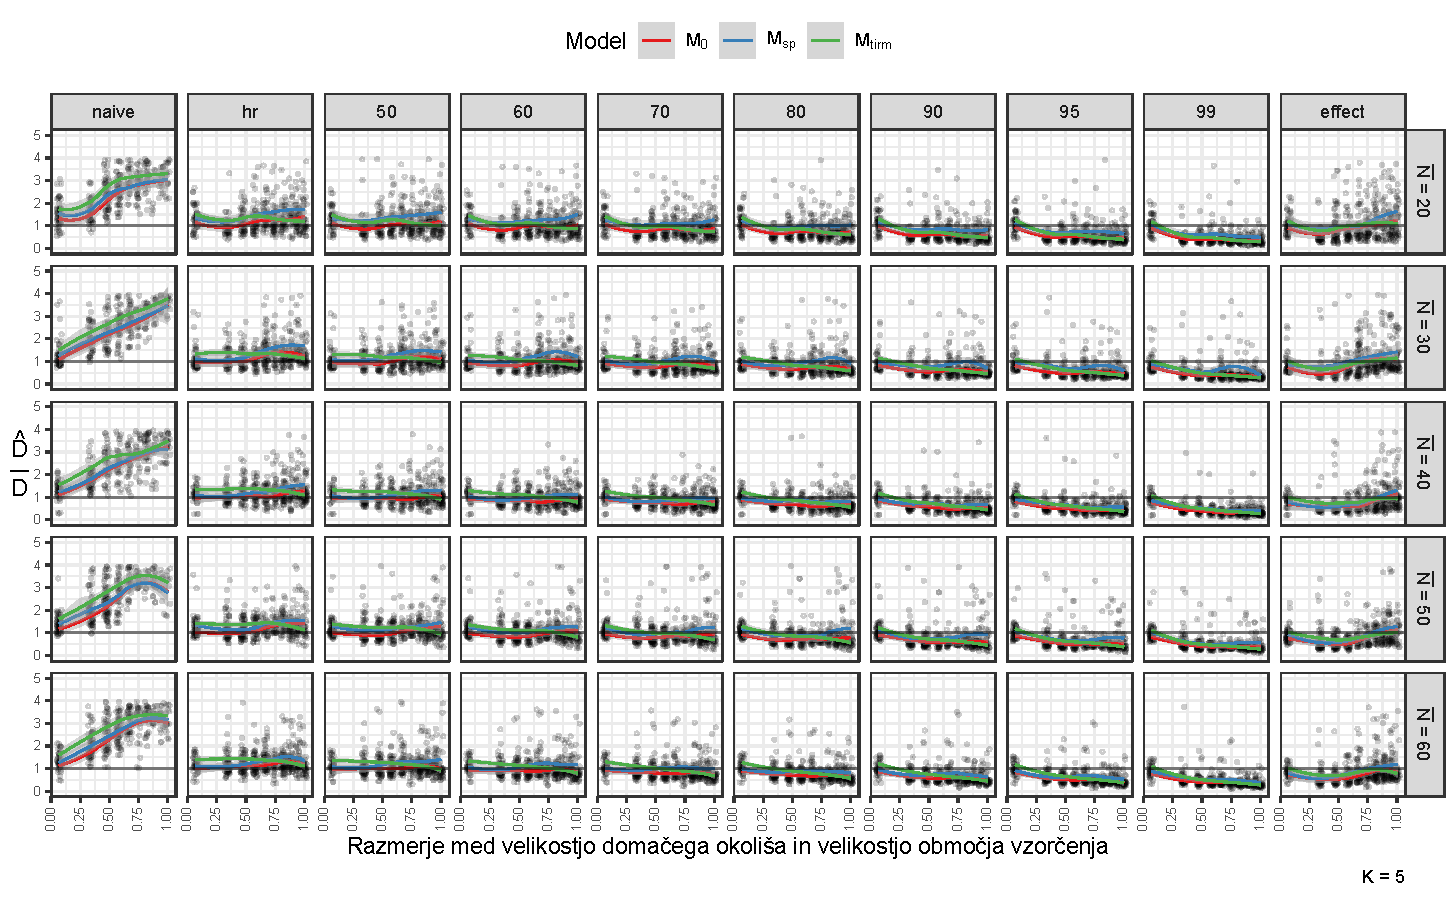
\includegraphics[width=1\linewidth]{C:/Users/romunov/Documents/workspace/doktorat/analiza/figures/N-1c_gostota_gled_na_razmerje_hr_sap_po_correction_type_in_st_gen_walk_za_k5.pdf}
    \label{sli:sub9.1}
  \end{subfigure}

  \begin{subfigure}[b]{1\textwidth}
    \centering
    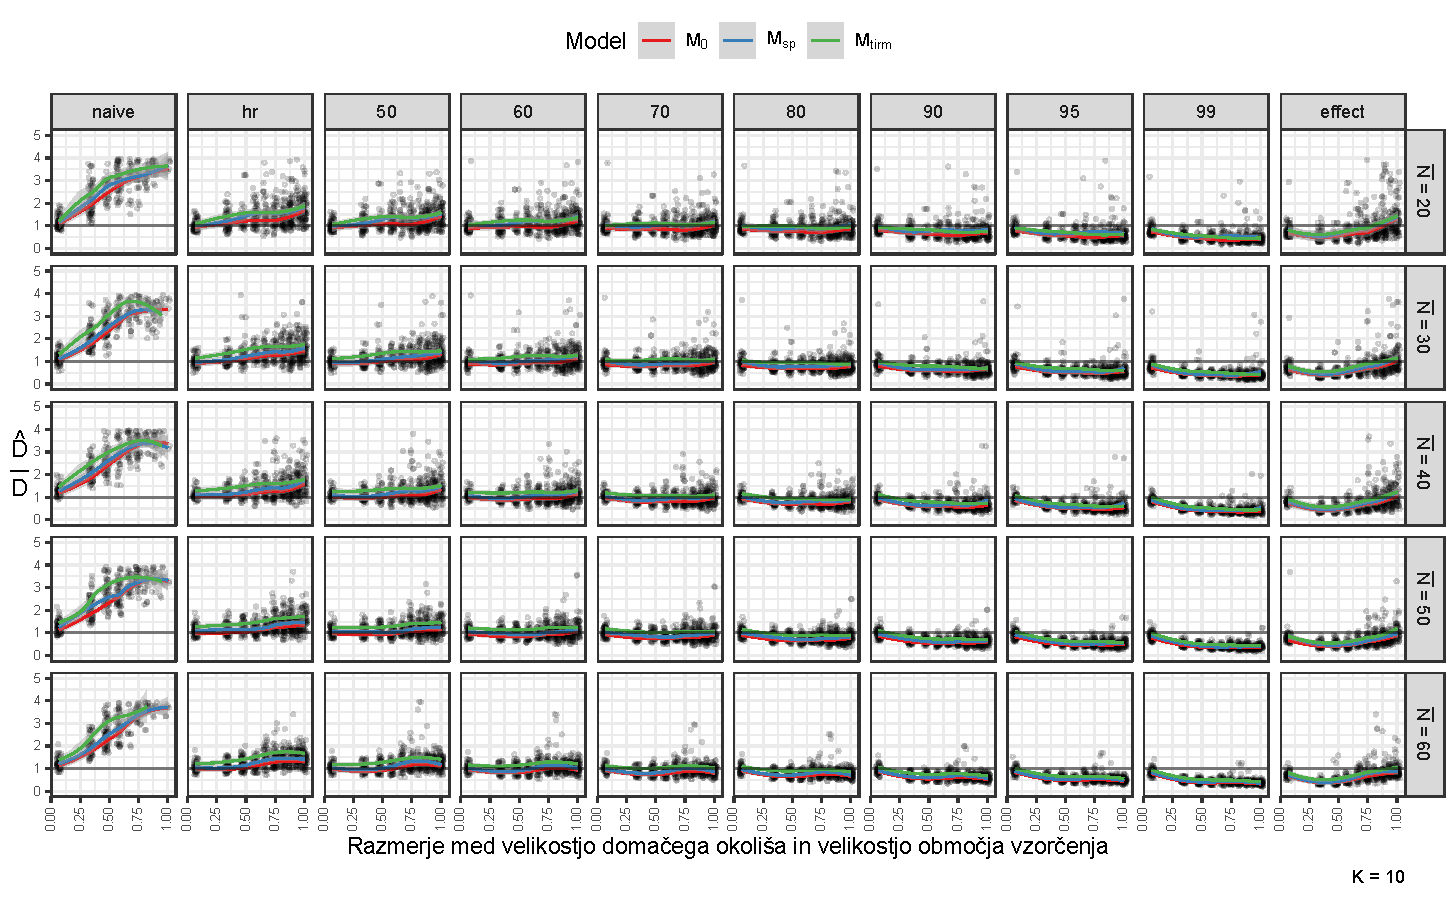
\includegraphics[width=1\linewidth]{C:/Users/romunov/Documents/workspace/doktorat/analiza/figures/N-1d_gostota_glede_na_razmerje_hr_sap_po_correction_type_in_st_gen_walk_za_k10.pdf}
    \label{sli:sub9.2}
  \end{subfigure}
\end{figure}

\begin{figure}[H]
  \ContinuedFloat
  \begin{subfigure}[b]{1\textwidth}
    \centering
    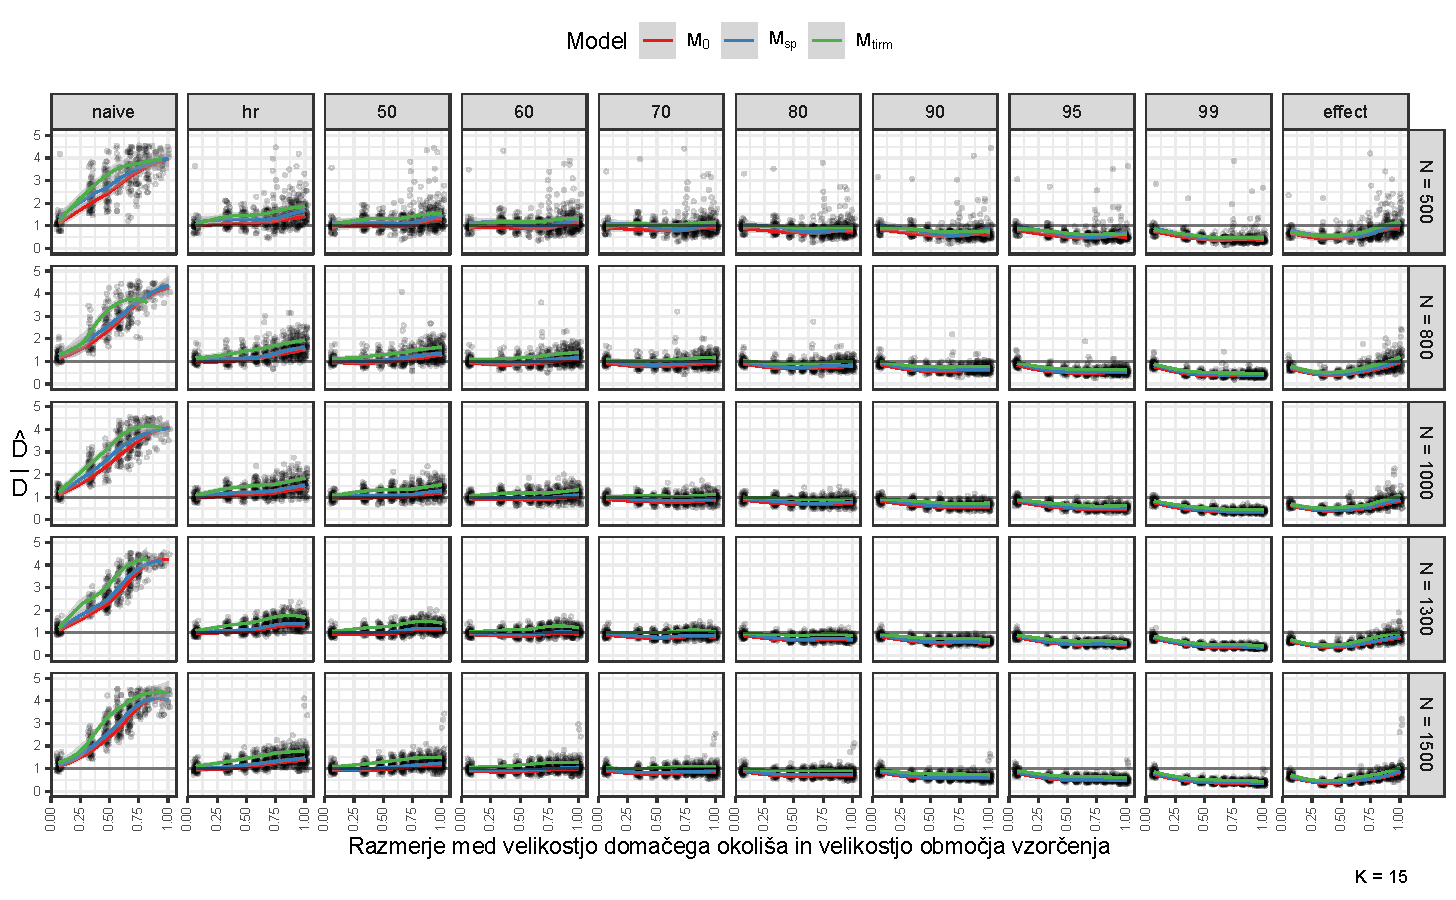
\includegraphics[width=1\linewidth]{C:/Users/romunov/Documents/workspace/doktorat/analiza/figures/N-1e_gostota_glede_na_razmerje_hr_sap_po_correction_type_in_st_gen_walk_za_k15.pdf}
    \label{sli:sub9.3}
  \end{subfigure}
  \caption[Prikaz vrednosti simulacij, kjer smo za izračun individualne spremenljivke uporabili normalno porazdelitev]{Prikaz vrednosti simulacij, kjer smo za izračun individualne spremenljivke uporabili normalno porazdelitev. Ta slika prikazuje iste podatke, kot so na sliki 8 (spodaj), dodatno pa smo jih razrezali glede na število odlovnih intervalov ($K$). Zgoraj $K=5$, v sredini $K=10$, spodaj $K=15$.}
  \label{sli:slika9}
\end{figure}

\subsection{AICc}
Metriko AICc smo primerjali samo za Hugginsova modela M0 in Msp. Verjetje modela TIRM ni primerljiv s Hugginsovim modelom. Poleg tega uporabi za izračun velikosti populacije drugačen set podatkov. Primerjava vrednosti AICc z ostalima dvema modeloma zato ne bi bila pravilna.

Za vsako simulacijo smo določili kateri model ima manjši AICc, nato pa razliko med modeloma prikazali na osi y. Vedno smo odšteli AICc modela M0 od AICc modela Msp. Negativne vrednosti so povezane s tistimi simulacijami, kjer je bil boljši model M0, pozitivne pa kjer je bil boljši model Msp. Če je bil boljši model Msp, je bila razlika pogosto mnogo večja (modra barva) kot v primerih, ko je bil boljši model M0 (rdeča barva). Število simuliranih osebkov ne vplivajo na razliko v AICc (ni prikazano), zato smo podatke prikazali brez te spremenljivke na sliki 10.

\begin{figure}[H]
  \centering
  \begin{subfigure}[b]{1\textwidth}
    \centering
    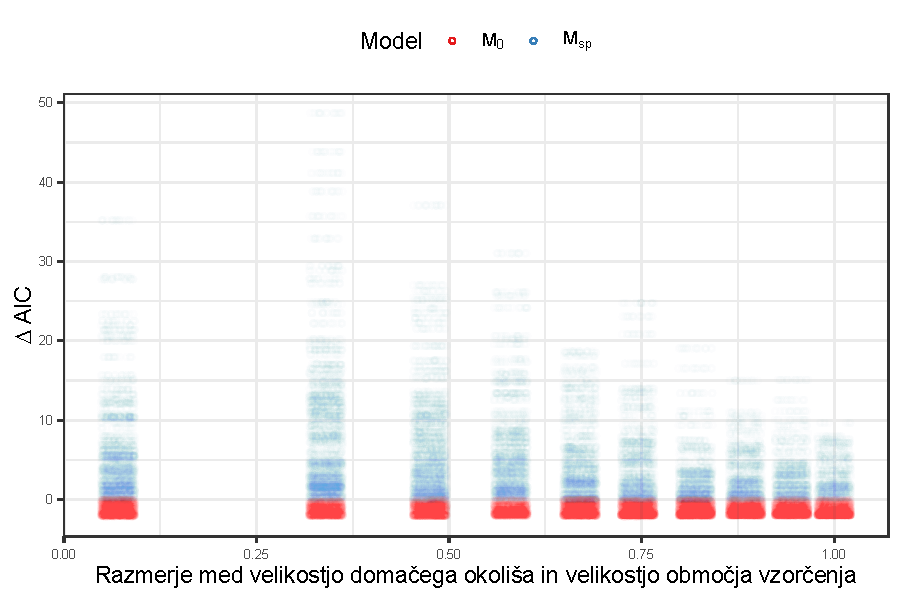
\includegraphics[width=1\linewidth]{C:/Users/romunov/Documents/workspace/doktorat/analiza/figures/E-6b_dAIC_glede_na_razmerje_hr_sap_po_correction_type_in_st_gen_walk_in_boljsi_model.pdf}
    \label{sli:sub10.1}
  \end{subfigure}

  \begin{subfigure}[b]{1\textwidth}
    \centering
    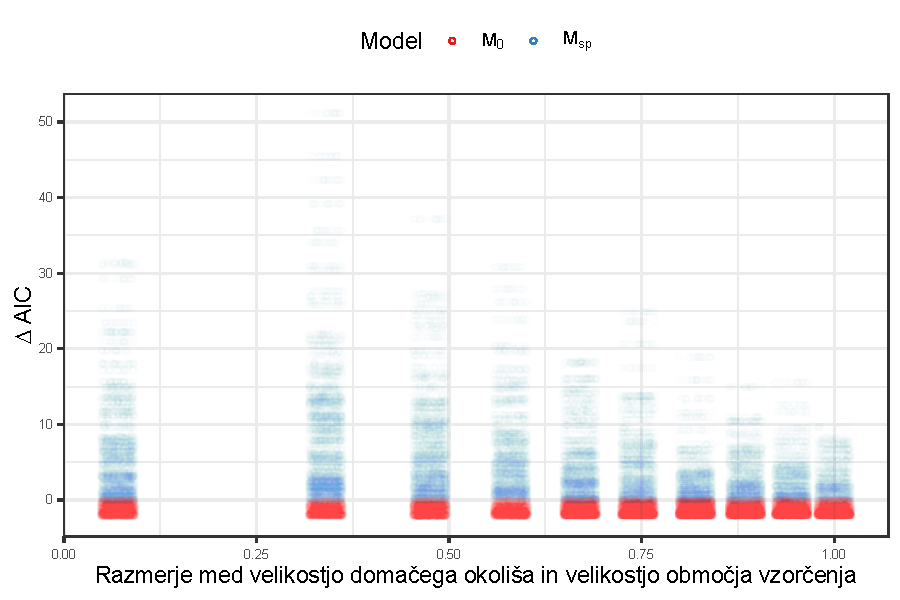
\includegraphics[width=1\linewidth]{C:/Users/romunov/Documents/workspace/doktorat/analiza/figures/N-6b_dAIC_glede_na_razmerje_hr_sap_po_correction_type_in_st_gen_walk_in_boljsi_model.pdf}
    \label{sli:sub10.2}
  \end{subfigure}
  \caption[Prikaz razlike v AICc za modela $M_0$ in $M_{sp}$]{Prikaz razlike v AICc za modela $M_0$ in $M_{sp}$. Na zgornji sliki so prikazani podatki, ker smo za izračun individualne spremenljivke uporabili empirično porazdelitev, na spodnji pa normalno porazdelitev. Rdeče obarvane točke predstavljajo simulacije, kjer je bil boljši model $M_0$, modre pa $M_{sp}$.}
  \label{sli:slika10}
\end{figure}

Porazdelitev vrednosti so nekoliko bolj razvidne s slike 11. Opazimo, da glede na to katero porazdelitev uporabimo za izračun individualne spremenljivke, v rezultatih ni razlik.

\begin{figure}[H]
  \centering
  \begin{subfigure}[b]{1\textwidth}
    \centering
    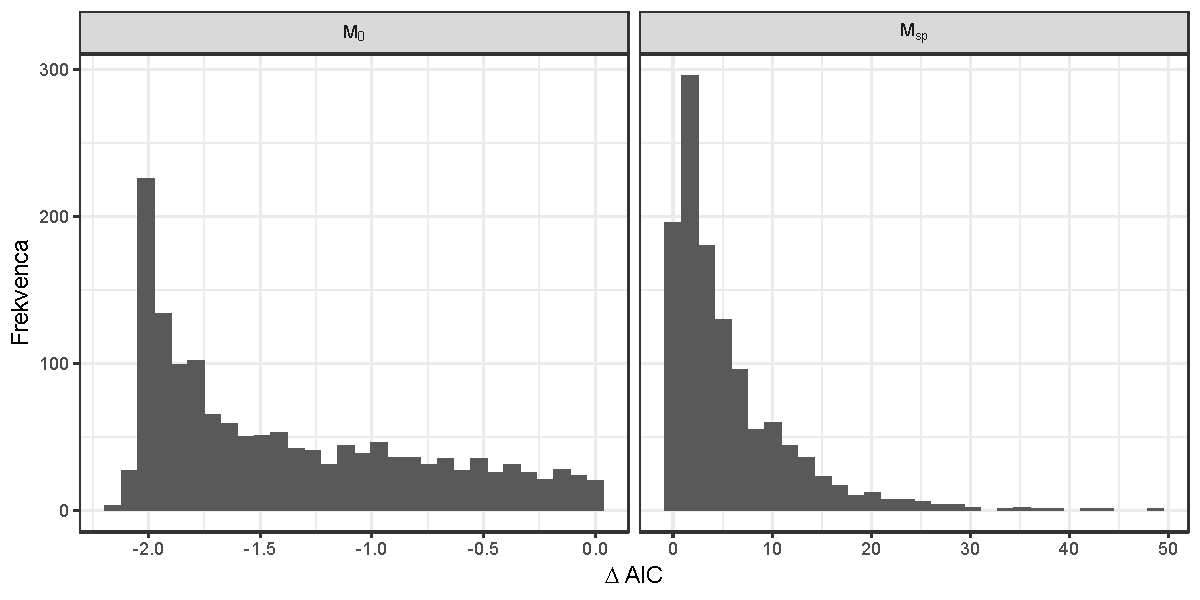
\includegraphics[width=1\linewidth]{C:/Users/romunov/Documents/workspace/doktorat/analiza/figures/E-8a_dAIC_glede_na_najboljsi_model.pdf}
    \label{sli:sub11.1}
  \end{subfigure}

  \begin{subfigure}[b]{1\textwidth}
    \centering
    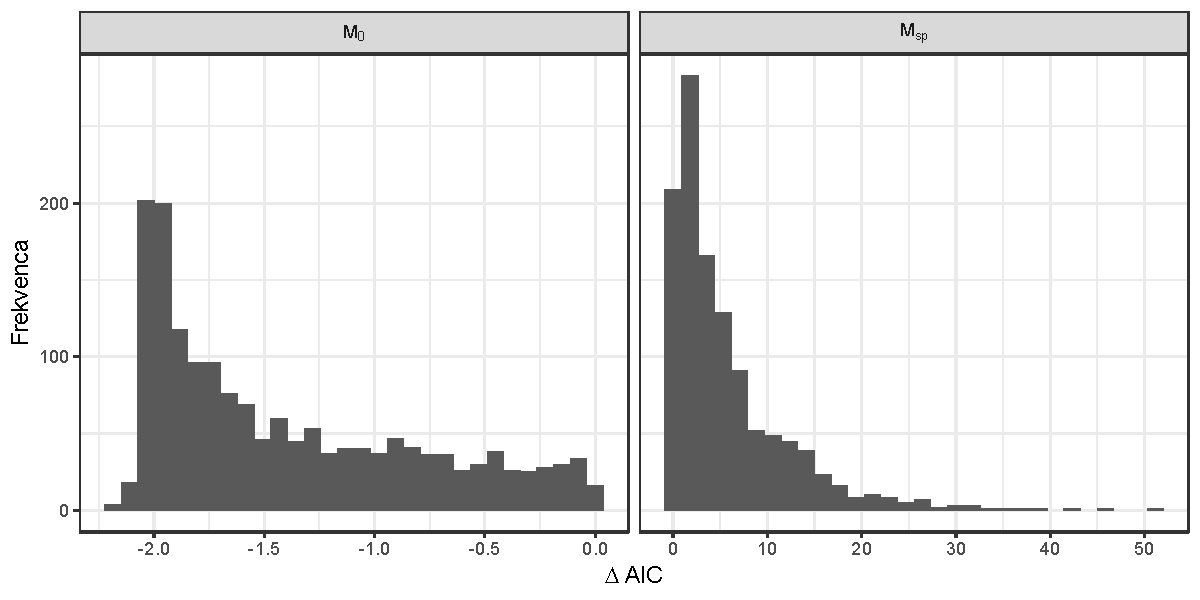
\includegraphics[width=1\linewidth]{C:/Users/romunov/Documents/workspace/doktorat/analiza/figures/N-8a_dAIC_glede_na_najboljsi_model.pdf}
    \label{sli:sub11.2}
  \end{subfigure}
  \caption[Prikaz razlike v AICc za modela $M_0$ in $M_{sp}$]{Porazdelitev razlik v AICc za modela $M_0$ in $M_{sp}$ s slike 10. Zgornja dva histograma predstavljata vrednosti, kjer smo za izračun individualnih spremenljivk uporabili empirično porazdelitev, spodnja dva pa normalno porazdelitev. Previdni morami biti  pri razlaganju osi x, saj le-ti med modeloma nista primerljivi.}
  \label{sli:slika11}
\end{figure}

\section{RAZPRAVA}
Pomembno orodje za raziskovanje nekaterih osnovnih parametrov populacij, kot je njena velikost, so metode lova-ponovnega ulova. Kot velja za vse metode, imajo tudi te nekatere predpostavke, ki nas do neke mere omejujejo. V tem delu smo se osredotočili na kršenje predpostavk zaprtosti populacije in enake verjetnosti ulovljivosti zaradi prihajanja in odhajanja osebkov v in iz območja vzorčenja. To prehajanje imenujemo učinek roba. Posledice učinka roba smo poskusili omiliti s popravkom, ki naj bi po našem mnenju opisoval ulovljivost osebkov v območju vzorčenja.

S pomočjo simulacij in klasičnih modelov za zaprte populacije (Hugginsov model) smo preverili delovanje predlaganega popravka. Vsakemu osebku smo izračunali individualno spremenljivko, ki je odvisna od lege vzorcev (centroida) v prostoru in predpostavljene funkcije gibanja. Gibanje okoli centroida smo opisali s pomočjo dveh porazdelitev. Prva je dvorazsežna normalna porazdelitev, za katero smo uporabili simuliran standardni odklon. Ta predstavlja t. i. ``zlati standard'', saj bi morala najbolje opisati gibanje osebkov. Druga porazdelitev pa je odvisna od premikov osebkov, katerim priležemo rahlo spremenjeno kumulativno porazdelitev Weibullove funkcije. Ta način ne zahteva dodatnih informacij, ki bi jih sicer lahko pridobili z dodatnimi metodami (npr. opremljanje osebkov s telemetrijskimi ovratnicami \citep{ivan-et-al-2013-aux}).

Opisovanje gibanja po (pol)normalni porazdelitvi je v simulacijskih študijah relativno pogosto \citep{bolker_ecological_2008, ivan_using_2013}, saj omogoča razumevanje gibanja in je hkrati (lahko) dovolj kompleksno, da opiše neke splošne lastnosti osebkov, kot se gibljejo v prostoru. Seveda pa je to poenostavitev, za katero ni nujno, da opiše gibanje osebkov dovolj dobro. Za bolj kompleksna gibanja raziskovalci uporabljajo realne podatke, ki jih naključno vzorčijo, in tako simulirajo gibanje osebkov (npr. \citealp{manning_estimating_2010}). Tako generirani podatki nam res dajo bolj realen opis gibanja, vendar pa je možno, da dobimo zaradi nereprezentativnega vzorčenja pristranske rezultate. Tak opis gibanja ni nujno prenosljiv med sezonami ali območji.

V tem delu smo primerjali različne scenarije, kjer smo spreminjali velikost domačega okoliša, število odlovnih intervalov, število simuliranih osebkov (gostoto) in ulovljivost. Velikost in obliko vzorčenega območja smo ohranjali konstantni, ker nas v simulacijah bolj zanima relativen odnos med velikostjo domačega okoliša in velikostjo območja vzorčenja. Rezultate simulacij smo primerjali s pomočjo treh modelov. Dva sta Hugginsova modela, $M_0$, kjer predpostavljamo enako ulovljivost vseh osebkov, in $M_{sp}$, kjer predpostavljamo, da se ulovljivost spreminja z individualno spremenljivko. Tretji model je TIRM, ki predpostavlja, da imajo osebki eno od dveh ulovljivosti.

\subsection{PRISTRANSKOST OCENE ULOVLJIVOSTI}
Ker območje vzorčenja ne zaobjame populacije v celoti, nekateri osebki prehajajo rob vzorčenja. Pri lovu v simulaciji smo v primeru, da smo tak osebek ujeli zunaj območja vzorčenja, ta vzorec krnili. Brez krnjenja bi bila ocenjena ulovljivost nepristranska, blizu simulirane vrednosti zaznavnosti. Ker pa smo točke, ki se niso nahajale znotraj območja vzorčenja krnili, smo to ulovljivost za robne osebke spremenili - jo zmanjšali. To je razvidno iz rezultatov (npr. slika \ref{sli:slika5}), kjer se odmik ocenjene ulovljivosti odmakne od simulirane, predvsem na račun velikosti domačega okoliša glede na velikost območja vzorčenja. Ko je domač okoliš relativno majhen, so te kršitve relativno majhne, a še vedno prisotne.

Ker gre za razmerje med ocenjeno in simulirano vrednostjo, so vrednosti bližje 1 bolj podobne simulirani vrednosti. Odstopanje od simulirane vrednosti je stalno glede na uporabljen model in je manjše za model $M_0$ (bližje pravi simulirani vrednosti) kot za model $M_{sp}$.
Prvi model je preprost, za vse osebke predpostavi enako ulovljivost in ``ne ve'', da so bili podatki krnjeni. Drugi model ``ve'', da smo podatke krnili, in do neke mere to poskuša nadoknaditi s pomočjo individualne spremenljivke. Ta spremenljivka naj bi opisovala pojav, ki spreminja ulovljivost osebka - v našem primeru opisuje, do kakšne mere osebki niso na voljo za vzorčenje zaradi prehajanja roba območja vzorčenja. V tem oziru kaže, da individualna spremenljivka izboljša model. Ocena se izboljša predvsem za simulacije z manj osebki in manj odlovnimi intervali. Razlika med modeloma je komaj opazna, ko pa število osebkov in število odlovnih intervalov povečujemo, razlik med modeloma praktično ni več.

Odstopanje od simulirane vrednosti je različno. Odstopanje za 75 \% ni nenavadno za tiste simulacije, kjer je bila površina domačega okoliša približno tako velika kot območje vzorčenja. S pomanjševanjem površine domačega okoliša relativno na površino območja vzorčenja (razmerje se manjša) pa se ta ocena izboljšuje in v najboljšem primeru odstopa le približno 25 \%. Zaradi krnjenja je manj verjetno, da bi ocenjene vrednosti v povprečju kadarkoli dosegle teoretično vrednost razmerja 1.

Iz razmerja ocenjene in simulirane ulovljivosti lahko opazimo, da se je variabilnost zmanjšala, ko smo povečali število odlovnih intervalov, nekoliko pa tudi zaradi večjega števila simuliranih osebkov. Manjša variabilnost je na račun tega, da smo v model vključili več podatkov. Takrat so ocene bolj natančne in je posledično ocena parametrov manj variabilna. Ta pojav nam je lahko v pomoč pri načrtovanju poskusa, kjer se odločamo, ali napor vložiti v večanje ulovljivosti osebkov, v večanje števila odlovnih intervalov ali obojega.

Kot osnovo, s katero smo primerjali rezultate modela $M_{sp}$, smo vzeli rezultate modela $M_0$, ki o osebkih ne predpostavlja drugega, kot da so vsi enako ulovljivi. Tak model je primeren za raziskave, kjer se osebki gibljejo samo znotraj območja vzorčenja. V naravi si lahko tak primer predstavljamo na primeru ribnika, kjer ribe ne morejo zapustiti območja vzorčenja in ima vsak osebek teoretično enako verjetnost ulova. Za primerjavo, model $M_{sp}$ preko individualne spremenljivke do neke mere upošteva kršenje predpostavke neprehajanja roba območja vzorčenja.

\subsection{PRIMERJAVA AICC ZA MODELA $M_0$ IN $M_{sp}$}
Primerjava modelov $M_0$ in $M_{sp}$ kaže, da ima slednji v povprečju konsistentno nižji AICc od prvega. V primerih, ko je boljši model $M_{sp}$, je razlika v AICc med obema modeloma okoli 10. Ko je model $M_0$ boljši, je razlika največ približno 2. Razlika v AICc 2 med dvema modeloma daje podporo tezi, da sta modela tako različna, da bi lahko tistega z nižjim AICc smatrali kot boljšega \citep{boulanger_corrigendum_2001}. Modeli, ki so v AICc za 10 in več boljši od drugega (imajo nižji AICc) imajo močno podporo, da so boljši od alternativnega modela \citep{burnham_model_2002}. Iz tega lahko sklepamo, da je model $M_{sp}$ v tem pogledu v povprečju zares boljši od $M_0$. Vendar je razlika v oceni parametra verjetnosti ulovljivosti $p$ za praktične potrebe majhna. Končni pokazatelj, ali je ta model res pomembneje boljši, je izračun gostote osebkov v območju vzorčenja, kar je navadno cilj raziskav.

\subsection{PRIMERJAVA OCEN GOSTOT}
Izračun gostote je za klasične raziskave lova-ponovnega ulova po svoje problematičen, ker je ključen del enačbe površina območja vzorčenja. Ocena velikosti populacije se nanaša na superpopulacijo, ki lahko prehaja rob vzorčenega območja, ni pa popolnoma znano, kolikšno je to prehajanje roba. Taka ocena gostote je zato pristranska, če ne poznamo mej območja, s katerega prihaja superpopulacija. Ta problem je reševal že \citet{dice_census_1938}, tako da je območje vzorčenja razširil za polmer domačega okoliša. Na podoben način so problem poskušali reševati vsi kasnejši raziskovalci \citep{williams_analysis_2002}.

Naš popravek spada med t. i. ad hoc pristope, kot jih kritizirajo \citet{royle_spatial_2013}. Klasični pristopi po večini lovijo na mreži pasti in statistike, ki jih je moč izluščiti iz takih podatkov, so navadno na mnogo bolj grobi skali, ki jo določa razmak med pastmi. Za razliko od klasičnih pristopov, ki beležijo samo ulov oz. neulov, lahko iz podatkov, nabranih zvezno v prostoru, izluščimo tudi točne lokacije ulovov. Ob zadostnem številu točk lahko sklepamo na velikost (in obliko) povprečnega domačega okoliša. To informacijo uporabimo, da izračunamo individualno spremenljivko, ki ponazarja verjetnost, da osebek ujamemo znotraj vzorčenega območja. Osebki, ki se nikoli ne približajo robu območja vzorčenja, imajo to vrednost 1, vsi ostali pa manj, odvisno od tega, kako daleč od roba se nahaja centroid domačega okoliša in kakšna je njegova oblika.

\subsubsection[\bfseries Računanje gostote brez popravka]{Računanje gostote brez popravka}
Ko smo izračunali gostoto brez popravka velikosti območja vzorčenja, tako da smo oceno velikosti populacije delili s površino vzorčenega območja, je bila ocena vedno precenjena za vsa razmerja med velikostjo domačega okoliša in območja vzorčenja in za vse modele ($M_0$, $M_{sp}$ in TIRM). Precenjena je na račun tega, da metoda lova-ponovnega ulova ocenjuje superpopulacijo \citep{white_capture-recapture_1982}, katere osebki prehajajo območje vzorčenja.

To je tudi razlog, da se raziskovalci odločajo za popravek velikosti območja vzorčenja. Popravek je še posebej potreben v primerih, ko se s populacijo aktivno upravlja in bi jo prevelik odvzem lahko pahnil v spiralo izumiranja.

Na variabilnost ocen imata velik vpliv število odlovnih intervalov in število generiranih osebkov, ne glede na to, s katerim modelom smo ocenili velikost populacije. To verjetno ni presenetljivo, saj z več odlovnimi intervali oz. osebki v model vključujemo več podatkov, zaradi česar je ocena bolj natančna.

\subsubsection[\bfseries Računanje gostote s pomočjo popravljene velikosti območja vzorčenja]{Računanje gostote s pomočjo popravljene velikosti območja vzorčenja}
Poleg naivne gostote smo izračunali tudi gostoto, kjer smo območja vzorčenja povečali za določeno razdaljo. Za izračun te razdalje smo histogramu parnih razdalj posameznih osebkov prilegli triparametrično Weibullovo porazdelitev oz. smo predpostavili normalno porazdelitev z vrednostjo standardnega odklona iz simulacije. Na podlagi teh porazdelitev smo določili razdaljo, ki sovpada s 50. do 99. percentilom prehojenih razdalj. Za dano razdaljo smo povečali premer, in s tem površino, vzorčenega območja. Območje smo razširili še za dve statistiki, simuliran polmer domačega okoliša (hr) in najdaljšo prehojeno razdaljo v simulaciji (effect).

Ocenjena gostota je za posamezen model ($M_0$, $M_{sp}$ in TIRM) konsistentna glede na razmerje med površino domačega okoliša in območja vzorčenja. To pomeni, da kažejo rezultati podobna gibanja glede na spremenljivke (število odlovnih intervalov, število generiranih osebkov, razširitev območja vzorčenja) in v odnosu do drugih modelov v vseh scenarijih. Model TIRM je najbolj precenjeval gostoto, vendar so te razlike za vse popravke v primerjavi z naivno gostoto relativno majhne.

Na sliki \ref{sli:slika6}, kjer sta prikazana oba načina računanja individualne spremenljivke, lahko vidimo, da se natančnost ocene modelov spreminja glede na število generiranih osebkov \citep{eberhardt_using_1990}. Ta učinek je še posebej viden na slikah \ref{sli:slika7} in \ref{sli:slika8}, kjer podatke prikažemo še glede na odlovne intervale. Večje število odlovnih intervalov vpliva na natančnost ocene, ker smo v model prek več odlovnih intervalov vključili več podatkov. Ta učinek je viden šele po tem, ko območje vzorčenja razširimo za katero koli mero.

Modela $M_0$ in $M_{sp}$ dajeta glede na simulirane spremenljivke (število odlovnih intervalov, število generiranih osebkov, razširitev območja vzorčenja) podobne rezultate in bi težko zagovarjali, da je v tem pogledu eden boljši od drugega. Razlike opazimo pri naivni gostoti, kjer TIRM model navadno ocenjuje nad Hugginsovima modeloma ($M_0$ in $M_{sp}$), ki sta si relativno podobna. Ko območje vzorčenja razširimo, se razlike med Hugginsovima modeloma nekoliko zabrišejo.

Bolj kot povečamo površino območja vzorčenja glede na domač okoliš osebka, manjše so razlike v oceni gostote med modeloma $M_0$ in $M_{sp}$. Naivno ocenjena gostota je najbolj pristranska in je v primerih, ko je razmerje med površino domačega okoliša in površino območja vzorčenja relativno veliko, precenjena tudi do 4-krat. To kaže, da je ocena gostote brez razmisleka o kršenju predpostavk lahko napačna, kar je pri upravljanju s prosto živečimi populacijami lahko problematično. Ker gre za precenjevanje, je treba odločevalcem pri podajanju rezultatov poudariti, da gre za optimistično oceno.

Ko območje vzorčenja razširimo za velikost simulirane velikosti domačega okoliša (en standardni odklon od centroida glede na normalno porazdelitev), se površina, s pomočjo katere računamo gostoto, poveča in posledično se ocena gostote in pristranskost zmanjšata. Najbolj točna ocena in relativno nepristranska za vse modele je okoli razširitve območja vzorčenja za 60. in 70. percentil. Če območje povečamo preveč, je ocena gostote lahko podcenjena. To velja za primere, ko za izračun individualne spremenljivke in posledično razdaljo za razširitev območja vzorčenja uporabimo znano, simulirano vrednost, ki opisuje gibanje osebkov in je t. i. ``zlati standard''. Ko območje vzorčenja razširimo za razdaljo med 60. in 70. percentilom normalne porazdelitve, zaobjamemo velik delež območja, ki ga zasedajo osebki, ki imajo centroid gibanja blizu roba območja vzorčenja. To bi približno sovpadalo s polovico premera velikosti domačega okoliša, kot je to predlagal \citet{dice_census_1938}.

Za naš popravek smo uporabili še empirično porazdelitev, ki smo jo prilegli podatkom - histogramu razdalj med pari točk. Percentil iz posamezne porazdelitve smo uporabili za izračun povečanja območja vzorčenja in izračun individualne spremenljivke.

Funkciji (empirična in normalna) se rahlo razlikujeta in razdalje pripadajočim percentilom niso identične. Empirična porazdelitev hitreje upade proti vrednosti 0 kot normalna. To je pričakovano, saj smo parametre za to porazdelitev ocenili iz vzorca lokacij osebka (za normalno porazdelitev smo uporabili simuliran standardni odklon). Podoben učinek opazimo pri metodi zankanja, ki navadno daje manjše intervale zaupanja statistik v primerjavi s parametričnimi metodami \citep{hesterberg_what_2015}. Empirična porazdelitev je tako le ocenjen približek iz podatkov. Ta ugotovitev nam služi kot varovalka, da se zavedamo, da so podatki le manjši izsek realnosti in ni nujno, da odražajo pravo stanje.

Za normalno porazdelitev tako poznamo pravo gibanje, stohastičen je samo položaj centroida domačega okoliša. Razlike, ki jih vidimo med modeloma $M_0$ in $M_{sp}$, lahko pripišemo razlikam funkcij, ki jih uporabimo za računanje individualne spremenljivke. Odstopanje centroida, izračunanega na podlagi vzorčenih točk od simuliranega gre pripisati vzorčenju majhnega števila točk.

Razlike v AICc med modeloma $M_0$ in $M_{sp}$ so primerljive s tistimi za normalno porazdelitev. Vpliv števila odlovnih intervalov ($K$) je podoben kot za normalno porazdelitev, kjer se varianca ocene gostote manjša z večanjem števila odlovnih intervalov.

Popravljanje gostote s širjenjem velikosti domačega okoliša sicer pomaga pri bolj pravilni oceni gostote, a šele ko območje vzorčenja povečamo za 80. percentil empirične porazdelitve (slika \ref{sli:slika8}). Pristranskost je, tako kot za normalno porazdelitev, relativno majhna za primere, kjer je razmerje med velikostjo domačega okoliša in območja vzorčenja relativno majhno (relativno majhen učinek roba). Pri povečanju za 90. percentil in več že prihaja do podcenjevanja ocene gostote. Najbolj točni so rezultati za simulacije z robnimi parametri - za največja in najmanjša razmerja med velikostjo domačega okoliša in območja vzorčenja. Podcenjevanje je z vidika upravljanja verjetno bolj zaželeno kot precenjevanje, ker daje zadržano oceno velikosti populacije.

Podatke smo simulirali s pomočjo normalne porazdelitve z znano varianco oz. standardnim odklonom. Ko smo računali individualno spremenljivko za posamezen osebek s pomočjo normalne porazdelitve, smo za vrednost standardnega odklona uporabili simulirano vrednost. Za popravek gostote smo območje vzorčenja razširili za razdaljo 60. percentila (približno en standardni odklon), kjer je bila gostota še najbližja simulirani. Z empirično porazdelitvijo smo to dosegli šele pri razširitvi območja vzorčenja za razdaljo 80. percentila. Iz tega bi lahko sklepali, da moramo območje povečati za določeno razdaljo, za katero, pa iz samih podatkov verjetno težko ocenimo. Morebitna rešitev bi bila z uporabo telemetrije (ali pridobimo podatek iz literature), kjer bi lahko območje vzorčenja povečali za toliko, da zajame večji delež domačih okolišev osebkov, ki so ob robu območja vzorčenja in še nezanemarljivo prispevajo k oceni številčnosti superpopulacije in gostote. Ta pristop ne bi potreboval izračuna individualne spremenljivke in so se ga poslužili že drugod \citep{ivan-et-al-2013-aux}. Nekateri sicer napovedujejo težve pri ocenjevanju parametra velikosti populacije v primeru heterogenosti ulovljivosti \citep{link_nonidentifiability_2003}, a glede na naše rezultate obstajajo primeri, ko napoved ni nujno tako slaba.

Popravek velikosti domačega okoliša bo najbolj koristil študijam, ki imajo opravka z vrstami z relativno velikim domačim okolišem (denimo medved \citep{miller_brown_1997, whittington_comparison_2015}), območje vzorčenja pa je relativno majhno. Če je območje vzorčenja znatno večje od velikosti domačega okoliša (npr. v primeru voluharjev \citealp{erlinge_density-related_1990}) in je torej razmerje blizu 0, popravek velikosti območja vzorčenja na gostoto ne bo imel bistvenega vpliva.

\newpage
\section{SKLEPI}
Ugotovili smo, da je model $M_{sp}$ z dodano individualno spremenljivko v povprečju boljši od modela, kjer spremenljivke nismo uporabili ($M_0$). Razlike v AICc so relativno velike (do približno 20) v prid $M_{sp}$. Le v nekaterih primerih je bil boljši model $M_0$, a so relativne razlike med modeloma razmeroma majhne (približno dve), do česar lahko pride že zgolj po naključju.

Ocenjeni ulovljivosti po modelu $M_{sp}$ in $M_0$ sta nižji od simulirane, kar pomeni, da zaznamo krnjenje zaradi prehajanja roba območja vzorčenja, s prvim modelom morda nekoliko bolje. Vendar pa so te razlike s praktičnega vidika zanemarljivo majhne.

Med ocenami gostote modelov $M_{sp}$, $M_0$ in TIRM nismo zaznali praktično pomembnih razlik. Z vključitvijo individualne spremenljivke v model $M_{sp}$ nismo uspeli za praktične potrebe izboljšati ocene gostote.

S pomočjo simulacij smo pokazali, da je razmerje med velikostjo domačega okoliša in velikostjo območja vzorčenja pomemben dejavnik pri proučevanju učinka roba. Z manjšanjem razmerja med velikostjo domačega okoliša in območja vzorčenja ($\rightarrow$ 0) se posledice učinka roba res zmanjšujejo. To se odraža na pristranskosti ocen parametrov ulovljivosti in posledično na velikosti populacije. Za večja razmerja ($\rightarrow$ 1) lahko do neke mere učinek roba popravimo s pomočjo podatkov, ki jih dobimo o velikosti domačega okoliša osebkov. Da bomo lahko zanesljivo popravili posledice učinka roba, bo potrebno oceniti velikost oziroma parametre funkcije domačega okoliša s pomočjo več podatkov (npr. telemetrija ali iz literature).

\section{Povzetek}

\section{Viri in reference}
\def\section*#1{}
\bibliographystyle{bib_style_bful}
\bibliography{ref_doktorat}

\section*{ZAHVALA}
\addcontentsline{toc}{section}{ZAHVALA}
\pagenumbering{gobble}

Doktorski študij je delno sofinancirala Evropska unija, in sicer iz Evropskega socialnega sklada. Sofinanciranje se izvaja v okviru Operativnega programa razvoja človeških virov za obdobje 2007-2013, 1. razvojne prioritete Spodbujanje podjetništva in prilagodljivosti; prednostne usmeritve\_1. 3: Štipendijske sheme.

Omenjeno sofinanciranje je bilo v obliki neobdavčenih 29.350,00 EUR. Odšteti gre še zneske, ki sem jih zapravil za priporočeno pošiljanje dokazil in bančnih potrdil na Univerzo.

Davnega leta 2008 me je za analizo podatkov v okviru diplomske naloge Jernej 'yerpo' Polajnar usmeril k programu \Q{R}. Program in skriptni jezik sta se mi dopadla in programiranje pozno v noč na domačiji Štelcar ni bilo nič nenavadnega. Pri analizi mi je bil v veliko pomoč Joris Meys z gentske univerze v Belgiji, ki je poskrbel, da nisem obupal že na začetku. Na srečo sem na Oddelku za biologijo našel še nekaj zanesenjakov in skupaj z Maartenom de Grootom in Majo Zagmajster smo ustanovili skupino navdušencev nad \Q{R}-jem, ki sem jo poimenoval \Q{R}koholiki. Na enem od srečanj je do mene pristopil Tomaž Skrbinšek in mi, še preden sem diplomiral, ponudil delo na projektu, ki ga je vodil Peter Trontelj. Z zamahom peresa sta mi dala edinstveno priložnost, da sem hobi zamenjal za poklic, kjer sem lahko programiral in si s tem še rezal kruh. Preko \Q{R}koholikov sem spoznal Ano Kolar, ki mi je namignila, da ``bi pa lahko vpisal doktorat iz statistike''. To je bilo verjetno prvič, da sem se sploh poigral z mislijo statistike. Leta 2011 sem vpisal doktorat. Hip hip strašen trik in projekta je končno konec. Pa hvala za vse ribe.

Veliko prijateljev mi je stalo ob strani in mi pomagalo v času doktorata. Težko bi poimensko omenil vse in jim naklonil pravično mesto med zvezdami digitalne univerzitetne knjižnice. Izpostavil pa bi svojo družino, ki mi je v dobrih in slabih časih brezkompromisno stala ob strani, za kar ji bom hvaležen do britofa. Hvala Mateji M za hitro in temeljito lektoriranje.

Brez vseh zgoraj naštetih in nenaštetih bi bil danes morebiti dosegljiv na telefonsko številko, ki jo imam v telefonu shranjeno pod ``A1 zaprti'' (01 587 22 67, Studenec 48, 1260 Ljubljana). Obljubim, da obstaja popolnoma racionalna razlaga, zakaj imam to številko shranjeno v telefonskem imeniku. Hvala.


\end{document}
